\documentclass[11pt]{article}

\usepackage{graphicx} % gere les images 
\usepackage[utf8]{inputenc} % pour les accents
\usepackage{hyperref} % pour les hyperliens
\usepackage[french]{babel} % langue fr
\usepackage{geometry} % pour les marges
\usepackage{listings} % pour le code
\usepackage{color}
\usepackage{enumitem} % permet de changer les listes a puces avec des rond
\usepackage{float}  % pour forcer les images a ce placer ou l'on veux avec l'option H
%\usepackage{here}  % pareil que float
\usepackage{array}
\usepackage{pdflscape} % pour passer en paysage

\title{L'affichage de l'enveloppe convexe dans le plan euclidien usuel} 
\author{Armen Mahmedov, Aurelien Patru} 
\date{\today} 

\hypersetup {
	colorlinks=true,
	linkcolor=black,
	urlcolor=red,
	citecolor=green,
	pdftitle={Initiation aux outils de simulation réseaux avec NS-2},
	pdfauthor={Armen,Aurelien},
	pdfsubject={simulation réseau avec NS-2},
	pdfkeywords={NS-2, réseau, nam, esirem, tcp, udp, }
}


% ################### Configuration partie code ########################### %
\definecolor{darkWhite}{rgb}{0.94,0.94,0.94}
\lstset{
	aboveskip=3mm,
	belowskip=-2mm,
	%backgroundcolor=\color{darkWhite},
	basicstyle=\footnotesize\ttfamily,
	breakatwhitespace=false,
	breaklines=true,
	captionpos=b,
	deletekeywords={...},
	escapeinside={\%*}{*)},
	extendedchars=true,
	keepspaces=true,
	%keywordstyle=\color{blue},
	literate=
	{²}{{\textsuperscript{2}}}1
	{⁴}{{\textsuperscript{4}}}1
	{⁶}{{\textsuperscript{6}}}1
	{⁸}{{\textsuperscript{8}}}1
	{€}{{\euro{}}}1
	{é}{{\'e}}1
	{è}{{\`{e}}}1
	{ê}{{\^{e}}}1
	{ë}{{\¨{e}}}1
	{É}{{\'{E}}}1
	{Ê}{{\^{E}}}1
	{û}{{\^{u}}}1
	{ù}{{\`{u}}}1
	{â}{{\^{a}}}1
	{à}{{\`{a}}}1
	{á}{{\'{a}}}1
	{ã}{{\~{a}}}1
	{Á}{{\'{A}}}1
	{Â}{{\^{A}}}1
	{Ã}{{\~{A}}}1
	{ç}{{\c{c}}}1
	{Ç}{{\c{C}}}1
	{õ}{{\~{o}}}1
	{ó}{{\'{o}}}1
	{ô}{{\^{o}}}1
	{Õ}{{\~{O}}}1
	{Ó}{{\'{O}}}1
	{Ô}{{\^{O}}}1
	{î}{{\^{i}}}1
	{Î}{{\^{I}}}1
	{í}{{\'{i}}}1
	{Í}{{\~{Í}}}1,
	morekeywords={*,...},
	framexleftmargin=16pt,
	framextopmargin=3pt,
	framexbottommargin=6pt,
	frame=td,
	numbers=left,    % numerotation
	numbersep=10pt,
	numberstyle=\tiny\color{black},
	stepnumber=1,
	rulecolor=\color{black},
	showspaces=false,
	showstringspaces=false, % don't mark spaces in strings
	showtabs=false,
	%stringstyle=\color{red},
	title=\lstname,
	keywordstyle=\color{red}\bfseries, 
 	commentstyle=\color{blue}\textit,
 	stringstyle=\color{cyan}\ttfamily,
 	tabsize=2,
 	frame=single % or td
}

% Pour changer les listings en Code
\renewcommand\lstlistingname{Script}
\renewcommand\lstlistlistingname{Script}

\setlist[itemize]{label=\textbullet} % pour tous les itemize changer le tiret avec un rond

\newcolumntype{M}[1]{>{\center}m{#1}} % definir un type de colone pour un tableau pour aller a la ligne  et etre centré
\newcolumntype{R}[1]{>{\raggedright}m{#1}}



\begin{document}

\begin{titlepage}
	\newcommand{\HRule}{\rule{\linewidth}{0.2mm}}     
            
	\begin{figure}[t]
		\begin{minipage}{0.5\textwidth}\large
			\begin{flushleft}
				
\includegraphics[width=0.7\textwidth]{assets/logoEsirem.jpg}
			\end{flushleft}
		\end{minipage}
		\begin{minipage}{0.5\textwidth}\large
			\begin{flushright}
			
\includegraphics[width=0.6\textwidth]{assets/logoUb.jpg}
			\end{flushright}
		\end{minipage}
	\end{figure}
	\textsc{ \\[1cm]}
     
     
	\begin{center}
	\HRule \\1
	{\Large   
		Initiation aux outils de simulation réseaux avec NS-2
	}
	\HRule
	\\[0.5cm]
	{\large Compte rendu tp reseau \\}
   \end{center}

	\begin{figure}[h]
		\begin{center}
			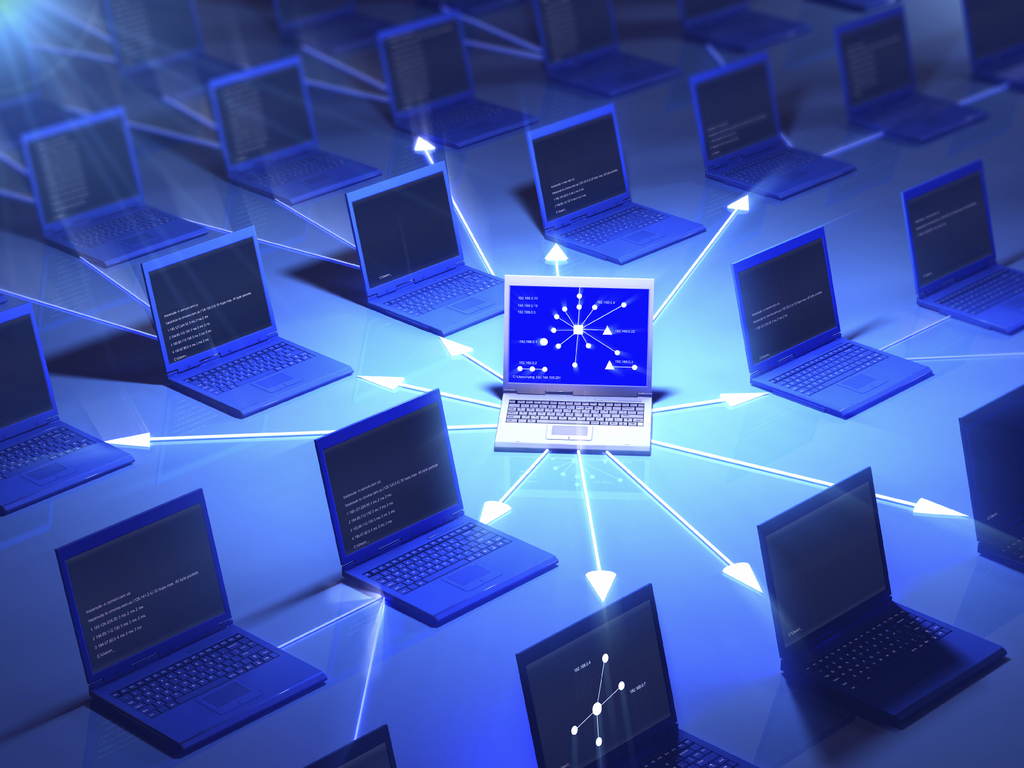
\includegraphics[width=0.5\textwidth]{assets/main.jpg}
		\end{center}
	\end{figure}
        
	\begin{center}
        \textsc{\large
        	ESIREM \\
			École Supérieure d'Ingénieurs de Recherche en Matériaux et en Infotronique\\       	
			[1.6cm]
		}
	\end{center}

	\begin{minipage}{0.5\textwidth}
		\begin{flushleft} \large
			\emph{Auteurs:}\\
			Armen Mahmedov \\
			Aurélien Patru
		\end{flushleft}
	\end{minipage}
	~
	\begin{minipage}{0.5\textwidth}
		\begin{flushright}\large
			\emph{Professeurs :} \\
			Nader Mbarek \\
			Ahmad Khalil
		\end{flushright}
	\end{minipage}
        
\end{titlepage}
  
% saut de page  ou   ~ \pagebreak 
\newpage
\strut
\newpage

%------------------------
%     Table des matieres
%------------------------
\tableofcontents

\pagebreak

%------------------------
%    Table des figures
%------------------------
\listoffigures

\pagebreak


\section*{Introduction}
\addcontentsline{toc}{section}{Introduction} 
NS (Network Simulator). est un logiciel libre de simulation à événements discrets très largement utilisé dans la recherche académique et dans l'industrie. L'utilisation d'un simulateur présente différents avantages comme par exemple celui de travailler sur un réseau et visualiser ses performances sans saturer le réseau. Il peut aussi être pratique d'utiliser un simulateur lors de la conception d'un réseau pour voir si, notre plan répond au besoin du client avant d'acheter et de tester dans un cas réel.

Ce compte rendu a pour but de synthétiser les trois travaux pratiques réalisés dans le module Réseau. Ils ont pour but l’utilisation et l’initiation de l’outil de simulation de réseaux NS-2. Dans un premier temps nous verrons la découverte de l'outil ns2 et nam puis on se focalisera sur le protocole de routage a vecteur distance puis sur le protocole à état de lien. Pour finir nous comment utiliser xgraph avec ns2 pour visualiser les performances d'un réseau.


\pagebreak


% Partie 1
\section{TP 1: Découvert de NS-2 et nam}
Dans ce premier TP nous allons apprendre à utiliser le logiciel de simulation NS-2. Pour cela, nous devons simuler un réseau simple à l’aide d’un script OTCL, mais également utiliser graphiquement le logiciel nam pour créer le même réseau. Puis dans un second partie nous devons simuler un réseau permettant la visualisation de congestion, perte de paquets et de pouvoir comparer le fonctionnement TCP (transmission Control Protocol) et UDP (User Datagram Protocol).

\subsection{Exercice 1: Simulation d'une topologie simple a deux noeuds avec un lien direct}

Dans un premier temps le but est de compléter le script fournis pour comprend se familiariser avec le langage et comprendre son fonctionnent

\subsubsection{Compléter le script}
Pour créer deux nœuds on utilise la commande \textbf{set}. Pour cela on peut soit créer les nœuds un par un soit le faire a l'aide d'un boucle for :

\begin{lstlisting}[language=tcl, numbers=none, framexleftmargin=0pt, framextopmargin=0pt, framexbottommargin=0pt]
set NodeNb 2
for {set i 0} {$i<$NodeNb} {set i [expr $i+1]} {set n($i) [$ns node]}
\end{lstlisting}

\noindent % pour ne pas faire d'alinea
Pour relier les deux nœuds on utilisera les paramètres suivants:
\begin{itemize}
	\item lien duplex de capacité 1MB
	\item temps de propagation de 10ms
	\item file d'attente de type DropTail
\end{itemize}

\begin{lstlisting}[language=tcl, numbers=none, framexleftmargin=0pt, 	framextopmargin=0pt, framexbottommargin=0pt]
$ns duplex-link $n(0) $n(1) 1Mb 10ms DropTail
\end{lstlisting}


Créer un agent UDP et l'attacher a n0. Ici la variable udp est une instance de la classe UDP qui hérite de la classe Agent

\begin{lstlisting}[language=tcl, numbers=none, framexleftmargin=0pt, 	framextopmargin=0pt, framexbottommargin=0pt]
set udp [new Agent/UDP]
#atacher l'aplication udp au noeud 0
$ns attach-agent $n(0) $udp 
\end{lstlisting}


Ensuite il faut créer une source de trafic CBR (\textit{constant bit rate}) avec les paramètres suivant:
\begin{itemize}
	\item taille des paquets de 500 octets
	\item intervalle de transmission de paquets de 0.005s
\end{itemize}

\begin{lstlisting}[language=tcl, numbers=none, framexleftmargin=0pt, 	framextopmargin=0pt, framexbottommargin=0pt]
#creattion d'un source de trafique
set cbr [new Application/Traffic/CBR]
$cbr set packetSize_ 500bytes
$cbr set interval_ 0.005s
\end{lstlisting}


Après avoir créer la source CBR, il faut maintenant le connecter a l'agent UDP avec la commande \textbf{attach-agent}
\begin{lstlisting}[language=tcl, numbers=none, framexleftmargin=0pt, 	framextopmargin=0pt, framexbottommargin=0pt]
#connecter le cbr a l'agent UDP
$cbr attach-agent $udp
\end{lstlisting}


Ensuite on doit créer l'agent null pour la réception des paquets dans le noeud 1 et connecter les deux agents Null et UDP
\begin{lstlisting}[language=tcl, numbers=none, framexleftmargin=0pt, 	framextopmargin=0pt, framexbottommargin=0pt]
#creation de l'agent null
set agentNull [new Agent/Null]
#atacher l'agent null au noeud 1
$ns attach-agent $n(1) $agentNull 
#connecter l'agent null et l'agent udp
$ns connect $udp $agentNull 
\end{lstlisting}

Il ne reste plus qu'à déclencher le trafic CBR à t=1s et l’arrêter à t=4.5s. Pour finir on doit arrêter la simulation après 5s. 
\begin{lstlisting}[language=tcl, numbers=none, framexleftmargin=0pt, 	framextopmargin=0pt, framexbottommargin=0pt]
#declancher le trafic cbf
$ns at 1 "$cbr start"
$ns at 4.5 "$cbr stop"
#Appeler la procédure de terminaison apres un temmps t 
$ns at 5.0 "finish"
#Executer la simulation
$ns run
\end{lstlisting}



\noindent
Le script complet se trouve l'annexe \ref{tp1Exo1}

\subsubsection{Visualisation de la simulation a l'aide de NAM}
Une fois le script complété on ouvre un terminal et on tape la commande \textbf{ns exercice1.tcl} pour compiler et lancer l'interface graphique nam que l'on peut voir dans la figure \ref{namVisu}. Cette commande crée aussi un fichier out.nam qui a été définit plus haut dans le script, plus tard si on veux revoir la simulation avec nam il suffira de lancer la commande \textbf{nam out.nam}


\subsubsection{Découvert des fonctionnalités de NAM}
L'utilitaire s'ouvre sur l'interface présentée en Figure \ref{namVisu}. Pour mieux comprendre le fonctionnement de nam on va détailler les différents parties présents en rouge sur la figure.

\begin{figure}[H]
	\begin{center}
		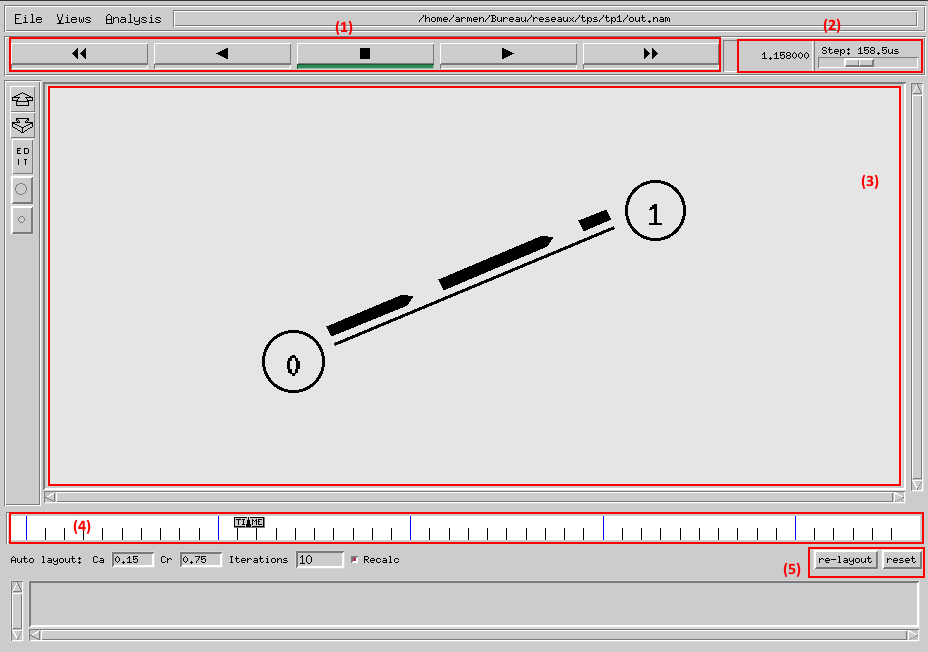
\includegraphics[width=0.7\textwidth]{assets/tp1/nam-visualisation1.png}
	\end{center}
	\caption{Interface nam pour la visualisation de la simulation}
	\label{namVisu}
\end{figure}

\noindent
(1) Sert a contrôler le déroulement la simulation \\
(2) Sert a visualiser le temps de la simulation et permet de contrôler sa vitesse\\
(3) Interface graphique ou la simulation se passe \\
(4) Permet de visualiser l'avancement de la simulation par rapport a la duré de la simulation et permet de se rendre directement un moment de la simulation\\
(5) Permet de changer la disposition des nœuds dans le cas ou les liens se croisent ou de reset la disposition des liens\\


Le logiciel nam permet a de nombreux fonctionnalités pour faciliter la compréhension du réseaux qui est actuellement simulé. Une des premières fonctionnalités disponibles avec cet outil est de pouvoir visualiser l’envoi de paquet comme on peut le voir dans la figure \ref{visuPaquet} Il est également possible si on clique sur le paquet de voir a quel moment il a été envoyé ainsi que sa taille. Ici dans notre exemple de la figure \ref{visuPaquet}, la taille du paquet est de 500 octets et il a été envoyé a 1.17s .

\begin{figure}[H]
	\begin{center}
		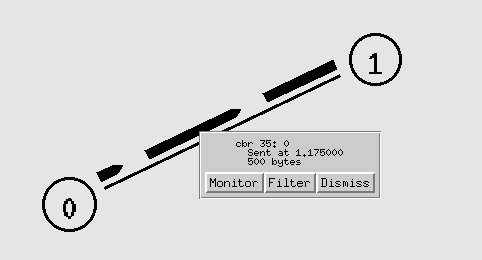
\includegraphics[width=0.7\textwidth]{assets/tp1/visualisationpaquet.png}
	\end{center}
	\caption{Visualisation en détail d'un paquet a l'aide de nam}
	\label{visuPaquet}
\end{figure}

On peut également avoir plus d'information (comme la bande passant ou encore le délais) sur un lien avec un clic, comme nous le montre la figure \ref{visuLien}.

\begin{figure}[H]
	\begin{center}
		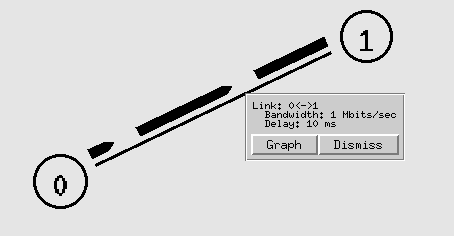
\includegraphics[width=0.7\textwidth]{assets/tp1/visualisationLien.png}
	\end{center}
	\caption{Visualisation en détail d'un lien a l'aide de nam}
	\label{visuLien}
\end{figure}

On peut également traquer un paquet en cliquant sur le bouton monitor alors cette paquet est affiche dans l'interface et on peut suivre son avancement


\begin{figure}[H]
	\begin{center}
		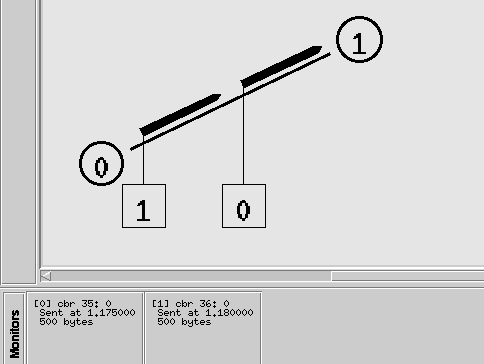
\includegraphics[width=0.7\textwidth]{assets/tp1/TraquerPaquet.png}
	\end{center}
	\caption{Traquer un paquet a l'aide de nam}
	\label{traquePaquet}
\end{figure}


\subsubsection{Utilisation graphique de NAM}

Maintenant il faut simuler le même réseau que dans la partie 1.1.1 mais cette fois avec l’interface graphique de nam. Pour cela nous allons tout d'abord faire une présentation rapide de l'interface graphique qui permet de créer la simulation. Pour lancer le logiciel il suffit de taper nam dans le terminal, ensuite il suffit d'aller dans fichier et cliquer sur nouveau éditeur nam,  l'utilitaire s'ouvre sur l'interface présentée en Figure \ref{namExplcation}.

\begin{figure}[H]
	\begin{center}
		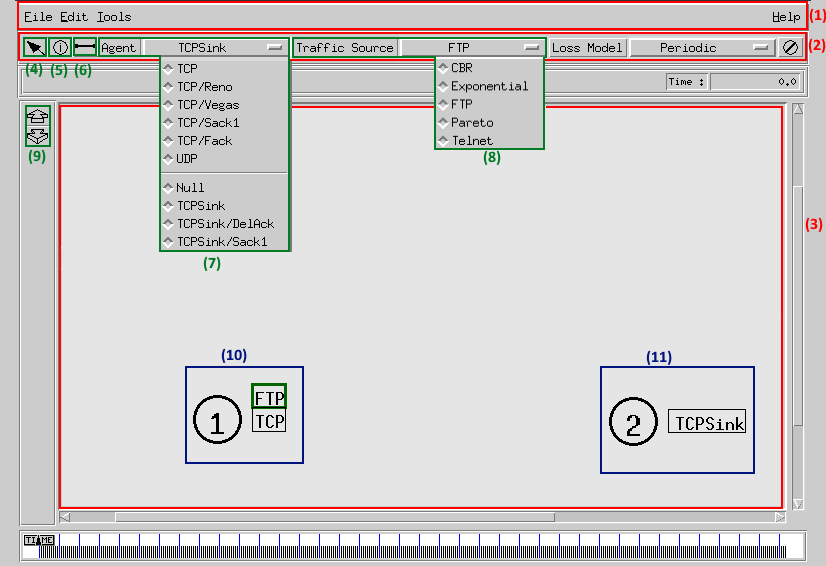
\includegraphics[width=0.8\textwidth]{assets/tp1/explicationNam.png}
	\end{center}
	\caption{L'interface graphique nam}
	\label{namExplcation}
\end{figure}

\noindent
(1) Le menu permettant d’accéder aux différents fonctions proposé par le logiciel\\
(2) Le menu d'action rapide qui permet d'avoir un raccourcis vers les fonctions présents dans le menu Tools\\
(3) L'interface graphique ou il faut placer les différents objets \\
(4) Le  curseur qui permet de sélectionner les objets et les bouger\\
(5) L'option qui permet de créer des nœuds\\
(6) Permet de faire le liens entre 2 nœuds ou 2 agents\\
(7) Permet de choisir un agent\\
(8) Permet de choisir une source de trafic \\
(9) Zoom/Dézoom\\
(10) Exemple de nœuds avec un agent TCP et une source de trafic FTP connecté a FTP\\
(11) Exemple de nœuds avec un agent TCPSink\\

Dans un premier temps on va créer 2 nœuds a l'aide du bouton ref(5) figure \ref{namExplcation}. Ensuite on les relis a l'aide du bouton ref(6) et avec in clic droit sur le lien on peut choisir le débit (Bandwidth), le temps de propagation (Delay) et la couleur du lien comme on peut le voir dans la figure \ref{ajoutLien}. Pour le type de file d'attente on peut le définir avec un clic droit le sur Q présent dans la figure \ref{ajoutLien}

\begin{figure}[H]
	\begin{center}
		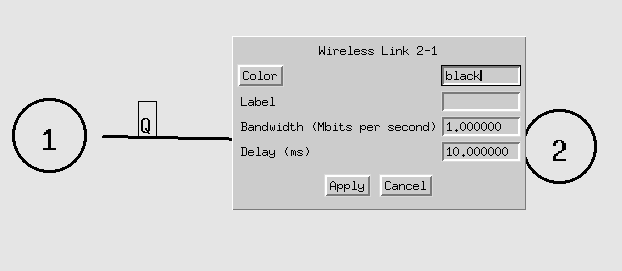
\includegraphics[width=0.6\textwidth]{assets/tp1/ajoutLienNoeud.png}
	\end{center}
	\caption{Ajout de lien entre 2 nœuds}
	\label{ajoutLien}
\end{figure}

Ensuite on crée l'agent UDP en sélectionnant dans le liste présent dans le ref(7) figure \ref{namExplcation} l'agent UDP et on cliquant sur le nœud 1. Pour pouvoir envoyer des informations il faut ajouter une source de trafic, ici on va ajouter une source CBR a notre agent UDP a l'aide du ref(8) figure \ref{namExplcation}, avec un clic droit sur la source on peut modifier l'intervalle de trasmission des paquets et quand le trafic doit se déclencher et s’arrêter comme on peut le voir dans la figure \ref{modifCBR}. Ensuite on va jouter l'agent Null au nœud 2 et connecter l'agent null avec l'agent UDP, après cette opération on peut modifier les options de UDP et changer la taille des paquets a 500 octets avec un clic droit sur l'agent UDP. Enfin pour modifier le temps de fin de simulation, il faut aller dans le menu \textit{Éditer} puis dans \textit{Propriétés du Simulateur}.

\begin{figure}[H]
	\begin{center}
		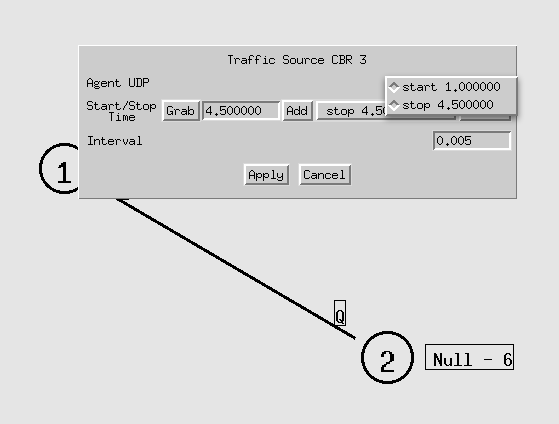
\includegraphics[width=0.6\textwidth]{assets/tp1/modifCBR.png}
	\end{center}
	\caption{Configuration source CBR}
	\label{modifCBR}
\end{figure}

La création de simulation avec l'interface graphique comporte quelques défauts comme par exemple la taille des paquets (packetSize) qui ne peut pas dépasser 210 octets alors qu'on les a fixer a 500.

\subsection{Exercice 2: Fonctionnement TCP vs UDP}

Dans cette exercice on s’intéresse au fonctionnement de TCP et UDP, pour cela on va simuler le réseau de la figure \ref{resSimu}.

\begin{figure}[H]
	\begin{center}
		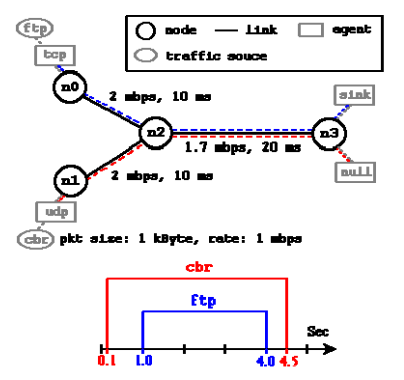
\includegraphics[width=0.6\textwidth]{assets/tp1/reseauAFaire.png}
	\end{center}
	\caption{Réseau à réaliser}
	\label{resSimu}
\end{figure}

Le script complet de cette exercice est disponible dans l'annexe \ref{tp1Exo2}. Par la suite nous ne détaillerons que les nouveaux éléments qui n'ont pas encore été abordé.

Pour réaliser ce réseau, on va tout d'abord créer 4 nœuds avec un boucle for, ensuite on les relis avec un lien duplex de capacité 2Mb avec un temps de propagation de 10ms pour les liens entre les nœuds n0 - n2 et n1 -n2 et un lien de 1,7Mb et un temps de propagation de 20ms entre n2 - n3, avec une file d'attente de type DropTail.
Par la suite on va créer 4 agent: 
\begin{itemize}
	\item TCP
	\item UDP
	\item Null
	\item TCPSink
\end{itemize}
L'agent TCPSink servira a communiquer avec le protocole TCP et l'agent Null avec le protocole UDP. De plus on va attacher l'agent TCP au nœud n0, UDP au nœud n1, TCPSink et Null au nœud n3. Ensuite on va créer 2 applications qui serviront a envoyer des données. L'application FTP qui sera connecté a l'agent TCP et le CBR à UDP.\\

Pour la partie configuration, on va limiter la taille du buffer entre n2 et n3 pour avoir une limité de 10 et pouvoir visualiser une congestion  avec la commande 
\begin{lstlisting}[language=tcl, numbers=none, framexleftmargin=0pt, 	framextopmargin=0pt, framexbottommargin=0pt]
$ns queue-limit $n(2) $n(3) 10
\end{lstlisting}

Pour l'agent CBR on va changer la taille des paquets a 1000 octets et un débit de 1Mb/s
\begin{lstlisting}[language=tcl, numbers=none, framexleftmargin=0pt, 	framextopmargin=0pt, framexbottommargin=0pt]
$cbr set packetSize_ 1000bytes
$cbr set rate_ 1Mb
\end{lstlisting}

Pour positionner les nœuds on va utiliser la commande \textbf{duplex-link-op}.
\begin{lstlisting}[language=tcl, numbers=none, framexleftmargin=0pt, 	framextopmargin=0pt, framexbottommargin=0pt]
#positionner les noeuds
$ns duplex-link-op $n(0) $n(2) orient right-down
$ns duplex-link-op $n(1) $n(2) orient right-up
$ns duplex-link-op $n(2) $n(3) orient right
\end{lstlisting}

Pour mieux visualiser et pouvoir distinguer les segments TCP et les datagrammes UDP on va les colorier, TCP en rouge et UDP en bleu.
\begin{lstlisting}[language=tcl, numbers=none, framexleftmargin=0pt, 	framextopmargin=0pt, framexbottommargin=0pt]
#déclaration de la couleur
$ns color 1 Red
$ns color 2 Blue

#affecter couleurs
$tcp set class_ 1
$udp set class_ 2
\end{lstlisting}



Pour finir on va lancer le trafic CBR à 0.1s et le terminer a 4.5s, le trafic TFP se lancera a 1s et se terminera a 4s

\begin{lstlisting}[language=tcl, numbers=none, framexleftmargin=0pt, 	framextopmargin=0pt, framexbottommargin=0pt]
#declancher le trafic cbf
$ns at 0.1 "$cbr start"
$ns at 4.5 "$cbr stop"
#declancher le trafic ftp
$ns at 1 "$ftp start"
$ns at 4 "$ftp stop"
\end{lstlisting}


Après la complication on se trouve dans nam qui compote notre simulation et on peut distinguer différentes étapes lors de son exécution.

\begin{enumerate}
	\item Envoie directe des données par UDP a 0.1s figure \ref{EnvoieUDP}
	
\begin{figure}[H]
	\begin{center}
		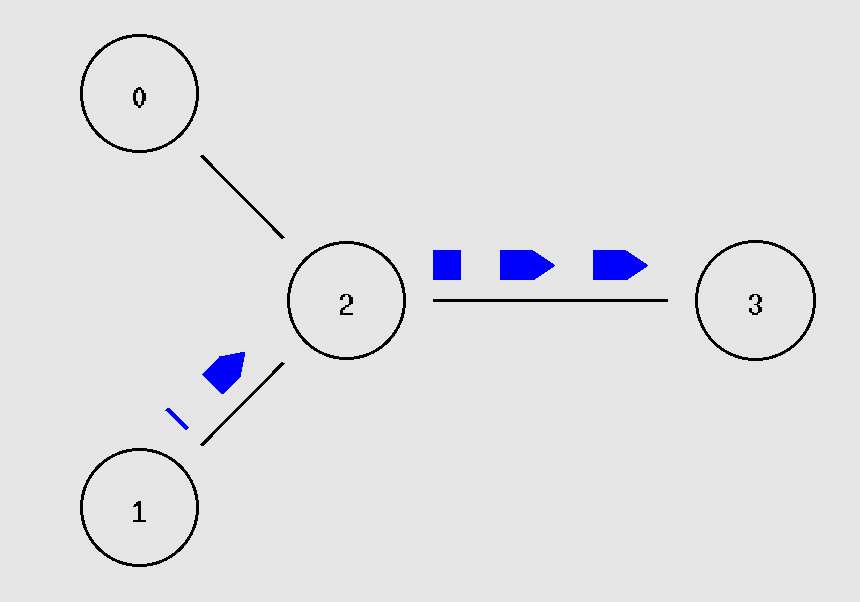
\includegraphics[width=0.6\textwidth]{assets/tp1/envoieDonneUDP.png}
	\end{center}
	\caption{Envoie de donné par UDP}
	\label{EnvoieUDP}
\end{figure}

	\item Envoie d'un demande de connexion par TCP à 1s (n0 demande à n3) figure \ref{demandeCo}. Le nœud n3 accepte la connexion figure \ref{acceptCo}
	
\begin{figure}[H]
	\begin{center}
		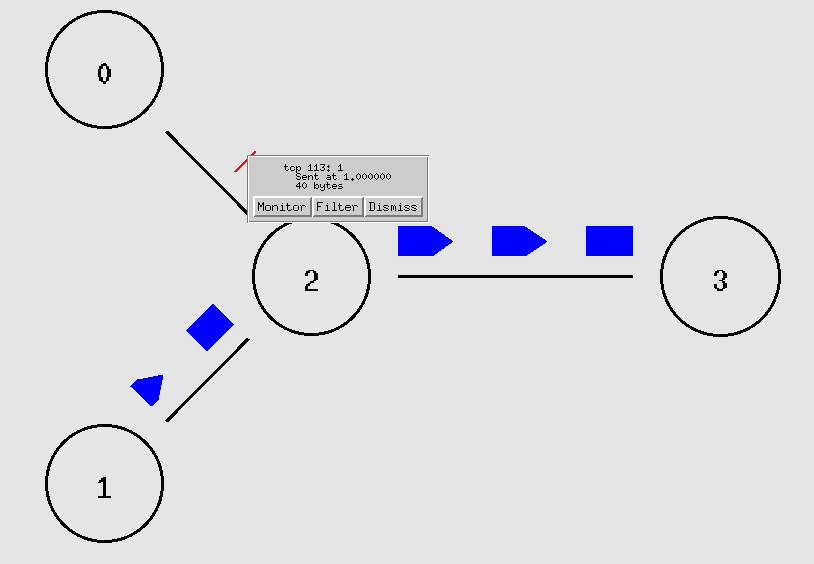
\includegraphics[width=0.6\textwidth]{assets/tp1/demandeDeCo.png}
	\end{center}
	\caption{Demande de connexion TCP}
	\label{demandeCo}
\end{figure}

\begin{figure}[H]
	\begin{center}
		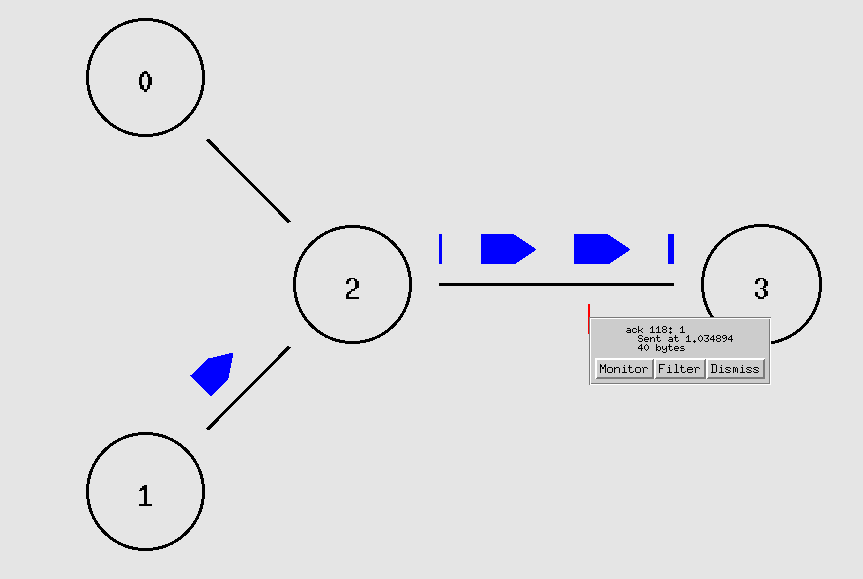
\includegraphics[width=0.6\textwidth]{assets/tp1/accepteCo.png}
	\end{center}
	\caption{Accepte demande de connexion TCP}
	\label{acceptCo}
\end{figure}

	\item Envoie des premiers segments TCP après l’établissement de la connexion. Ensuite envoie des segments seulement après acquittement figure \ref{acuseRecep}

\begin{figure}[H]
	\begin{center}
		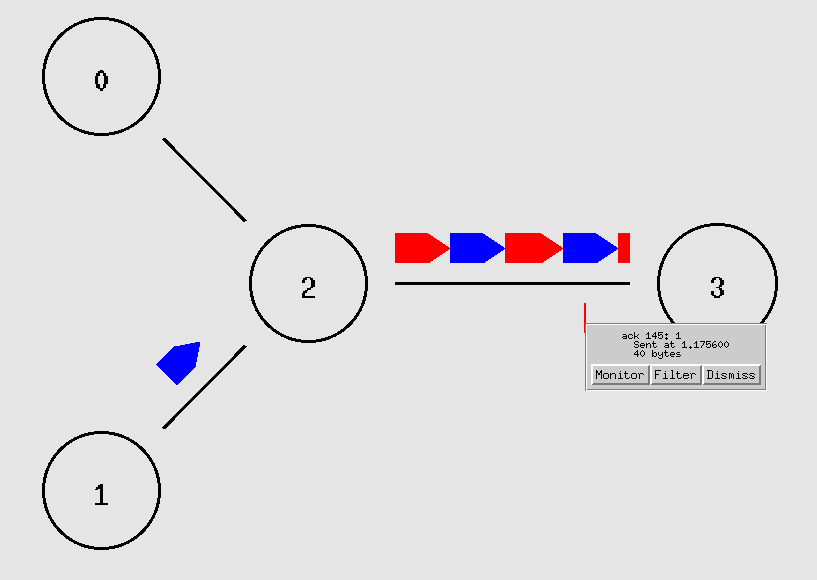
\includegraphics[width=0.6\textwidth]{assets/tp1/acuseReceptionPaquet.png}
	\end{center}
	\caption{Accusé de réception d'un paquet}
	\label{acuseRecep}
\end{figure}
	
	\item Congestion au niveau du nœud 2 avec drop de segment
	
\begin{figure}[H]
	\begin{center}
		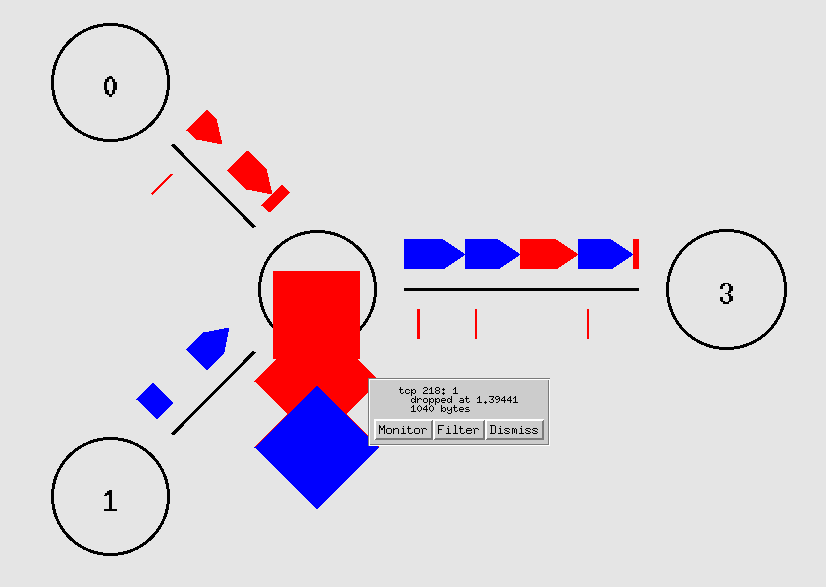
\includegraphics[width=0.6\textwidth]{assets/tp1/dropDePaquet.png}
	\end{center}
	\caption{Perte de paquet}
	\label{acuseRecep}
\end{figure}
	
	\item Après la perte des segments, UDP continu d'envoyer comme avant alors que TCP ayant détecté la perte 	réagit et diminue la quantité d’information envoyé, figure \ref{detectPaquete}

\begin{figure}[H]
	\begin{center}
		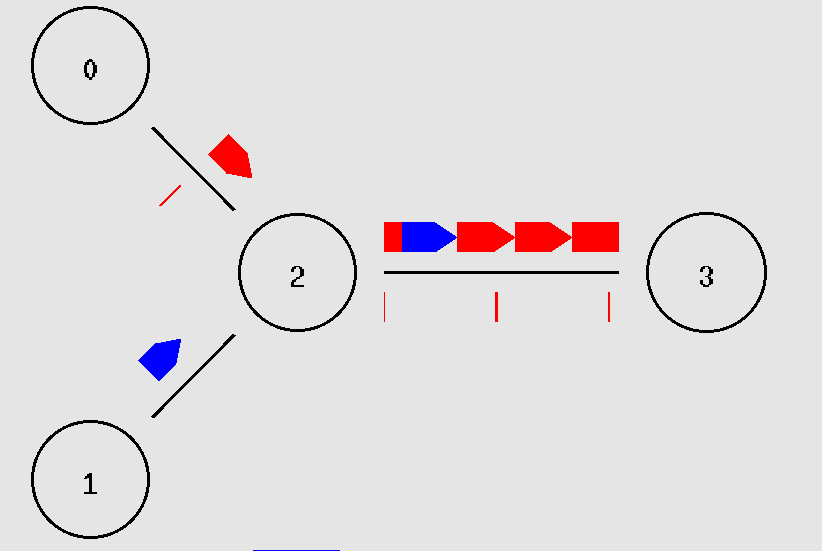
\includegraphics[width=0.6\textwidth]{assets/tp1/tcpDetectionPerte.png}
	\end{center}
	\caption{Détection de perte de la part de TCP}
	\label{detectPaquete}
\end{figure}
	
	
	
\end{enumerate}


Au départ TCP envoie que 2 segments, après l’acquittement de ces segments, TCP va doubler la taille de la fenêtre et envoyer 4 et ainsi de suite jusqu'au moment ou il détecte une perte de segment et va réagir en diminuant la quantité d'information envoyé pour s'adapter au capacité du réseau (contrôle de congestion) figure \ref{detectPaquete}. 

Au bout d'un moment nœud 2 reçoit trop d'information en même temps des nœuds n0 et n1 (4Mb/s) alors qu'il transmet qu'a 1.7MB/s, il est donc obligé de stocker les segments dans son buffer qui a une capacité limité (10). Quand le buffer du nœud n2 atteint sa capacité maximale le nœud commence a doper les paquets, on peut apercevoir ce comportement dans la figure 

~\\
\\
\\
\\
\\


% conclusion du grand 1
Pour conclure dans ce premier TP, nous avons pu nous familiariser avec l’outil de simulation NS-2. Avec tout d’abord la réalisation d'un réseau à l’aide d’un script OTCL permettant de découvrir le langauge et son fonctionnement, puis la visualisation la création de ce même réseau avec l'éditeur graphique nam permettant ainsi de se familiariser avec cette outil. Dans un deuxième temps nous avons pu comparer deux modes de communications (TCP et UDP) vu en cours pour mieux comprendre leur fonctionnement. Nous avons pu identifier le comportement de ces 2 modes de communication en cas de congestion ou encore visualiser l'envoie de données. Pour le protocole TCP nous avons visualisé l'envoie des segment TCP, la demande de connexion et l'acquittement. Pour le protocole UDP nous avons vu le mode non connecté et l'envoie de segment UDP (datagrame).

\pagebreak
% Partie 2
\section{TP 2: Protocole de routage de type Vecteur distance et Etat de liens}
Dans ce second nous allons voir deux types de protocoles de routage. Le but étant d’expérimenter les protocoles de routage à vecteur distance et à état de lien pour déceler leurs fonctionnements et particularités.

\subsection{Exercice 1: Comparaison des deux protocoles de routage}
Dans cette exercice on se propose de créer le réseau de la figure \ref{resAReal}
\begin{figure}[H]
	\begin{center}
		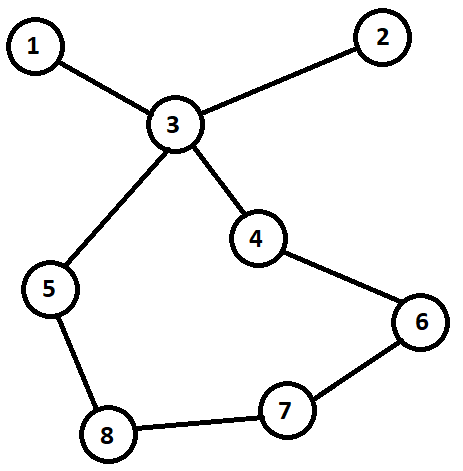
\includegraphics[width=0.6\textwidth]{assets/tp2/reasauRealiser.png}
	\end{center}
	\caption{Topologie du réseau a simuler}
	\label{resAReal}
\end{figure}


Tous d’abord avant de commencer l’analyse des résultats nous allons vous présenter la manière dont nous avons programmé cette simulation. Pour créer la simulation de cet exercice nous avons utilisé des commandes vues lors du tp1 ainsi que de nouvelles commandes que nous allons vous présenter ici. Le script complet est disponible dans l'annexe ************a faire(mettre code en annexe) ******** :

Tout d'abord on va créer 8 nœuds a l'aide de la commande vue dans le tp précédant, ensuite on s'occupe de la création des liens (avec la commande \textbf{duplex-link}) entre chaque nœud n(1) à n(8) avec un débit de 10Mb, un temps de propagation de 10 ms et une file d’attente de types DropTail. Pour ce réseau nous avons besoin de deux agents UDP, l’un pour le noeud n1 et l’autre pour le noeud n2, et deux sources CBR avec une taille de segment de 500 octets et 5 ms d’intervalle de transmission des paquets. Ensuite on va connecter les sources aux agents. On procède par la suite à la création de l’agent NULL pour la réception des paquets, et on l'attache au nœud n(8). On connecte ensuite udp1 et udp2 à l'agent Null. On attribut des couleurs au flux et on définit les débuts et fin de trafic. Et pour finir avec les commandes vues lors du tp1, on positionne ensuite les nœuds pour que le réseau ait l’apparence de la topologie demandé. 

\noindent
Nouvelles commandes :

- Définir le protocole de routage utilisé :\\
Pour définir le protocole de routage à utiliser nous avons utilisé la commande suivante :

\begin{lstlisting}[language=tcl, numbers=none, framexleftmargin=0pt, 	framextopmargin=0pt, framexbottommargin=0pt]
#DV: étant utilisé pour définir un protocole de routage à vecteur distance
$ns rtproto DV
#LS: étant utilisé pour définir un protocole de routage à état de lien
$ns rtproto LS
\end{lstlisting}

- Il nous a également fallut programmer la rupture du lien entre les nœuds 5 et 8 à 4s puis la reprise à 5s par les commandes suivantes :

\begin{lstlisting}[language=tcl, numbers=none, framexleftmargin=0pt, 	framextopmargin=0pt, framexbottommargin=0pt]
#rupture du lien à 4 secondes
$ns rtmodel-at 4.0 down $n(5) $n(8)
## rétablissement à 5 secondes
$ns rtmodel-at 5.0 up $n(5) $n(8)
\end{lstlisting}

Pour pouvoir comparer les deux protocoles de routage, on va écrire deux script, un avec un protocole de routage de type \textbf{vecteur distance} (DV) et l'autre à \textbf{état de lien} (LS). Pour cela les images a gauches seront pour le protocole vecteur distance et a droit pour état de lien.\\

Nous pouvons remarquer, que dès l’initialisation les protocoles sont différents. Pour le protocole vecteur distance (DV), il y a moins d’échanges de paquets que pour le protocole à état de lien (LS). 

En effet, pour le protocole DV, les nœuds ne possèdent pas une vision global du réseau, la diffusion des routes se fait de proche en proche comme on peut le voir dans le figure \ref{initDV}, par exemple le nœud 2 va envoyer que a ses voisin c'est à dire les nœuds 0,1,4 et 3. Donc au départ, chaque nœud n'as connaissance que des nœuds auquel il est directement connecté. 

Pour le protocole LS, les nœuds ont une vision global du réseau, ils construisent une carte complète de la topologie du réseau, ce qui peut expliquer que le nombre important d'échange de paquet lors de l'initialisation
que l'on peut voir dans la figure \ref{initLS}.

\begin{figure}[H]
    \begin{minipage}[c]{.5\linewidth}
        \centering
        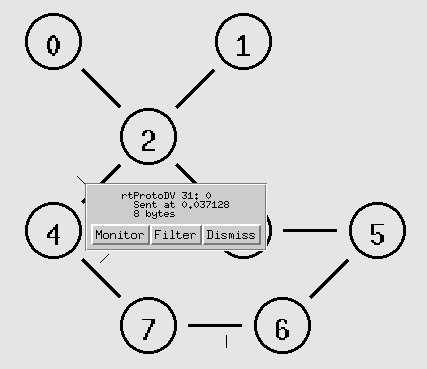
\includegraphics[width=0.9\textwidth]{assets/tp2/RoutageInitDV.png}
        \caption{Initialisation du routage DV}
        \label{initDV}
    \end{minipage}
    \hfill%
    \begin{minipage}[c]{.5\linewidth}
        \centering
        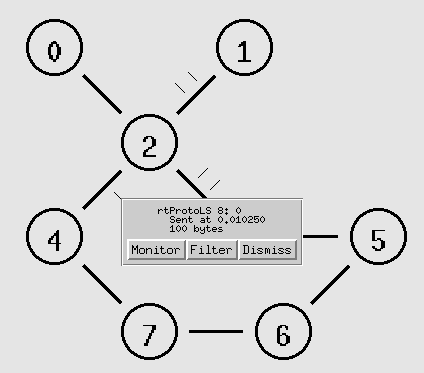
\includegraphics[width=0.9\textwidth]{assets/tp2/RoutageInitLS.png}
        \caption{Initialisation du routage LS}
        \label{initLS}
    \end{minipage}
\end{figure}

Lors de la rupture du lien entre les deux nœuds, nous pouvons remarquer que les protocoles
réagissent différemment.

Pour le protocole vecteur distance:

\begin{figure}[H]
	\begin{center}
		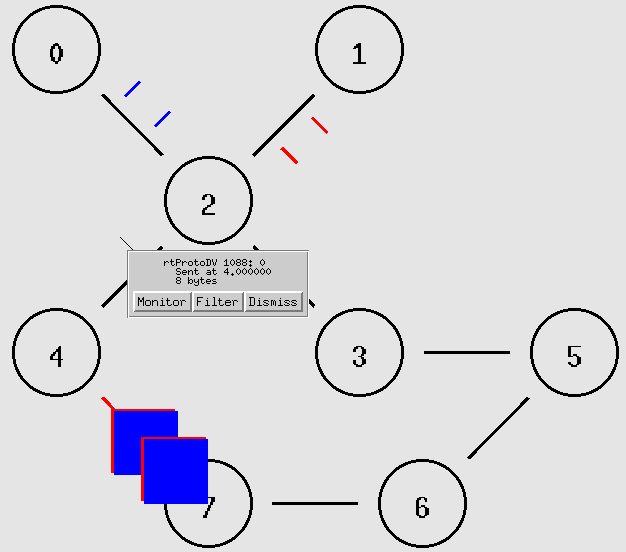
\includegraphics[width=0.6\textwidth]{assets/tp2/RutpureLienDV.png}
	\end{center}
	\caption{Réaction a une rupture de lien DV}
	\label{ruptureDV}
\end{figure}


Dans ce protocole, lors de la rupture de lien entre le nœud 4 et 7, un paquet est envoyé par le nœud 4 au nœud 2 pour l'informer de la rupture de lien comme nous le montre la figure \ref{ruptureDV}. Le temps que la détection se fasse tous les paquets envoyé par le nœud 2 au nœud 4 seront perdus. La rupture s’effectue à 4s et le prochain paquet qui prendra un chemin différent s'effectue à 4.03s comme nous le montre la figure \ref{detectRuptureDv}, donc la détection de la rupture de lien s’effectue 0.03s pour ce protocole.

\begin{figure}[H]
	\begin{center}
		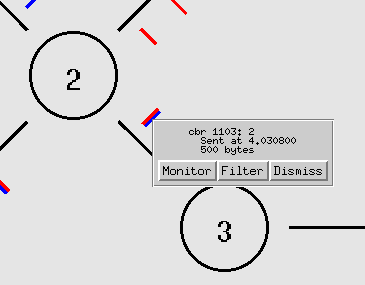
\includegraphics[width=0.5\textwidth]{assets/tp2/detectionRuptureDV.png}
	\end{center}
	\caption{Détection de la rupture de lien DV}
	\label{detectRuptureDv}
\end{figure}


Pour le protocole à état de lien:

\begin{figure}[H]
    \begin{minipage}[c]{.5\linewidth}
        \centering
        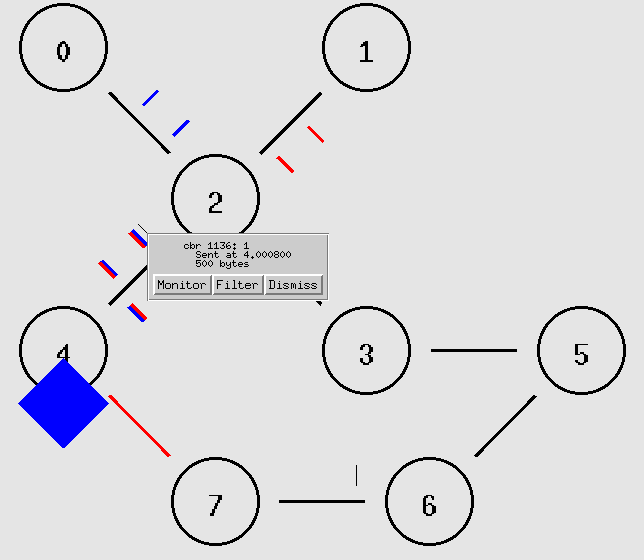
\includegraphics[width=0.9\textwidth]{assets/tp2/ruptureLS.png}
        \caption{Réaction a une rupture de lien LS}
        \label{ruptureLS}
    \end{minipage}
    \hfill%
    \begin{minipage}[c]{.5\linewidth}
        \centering
        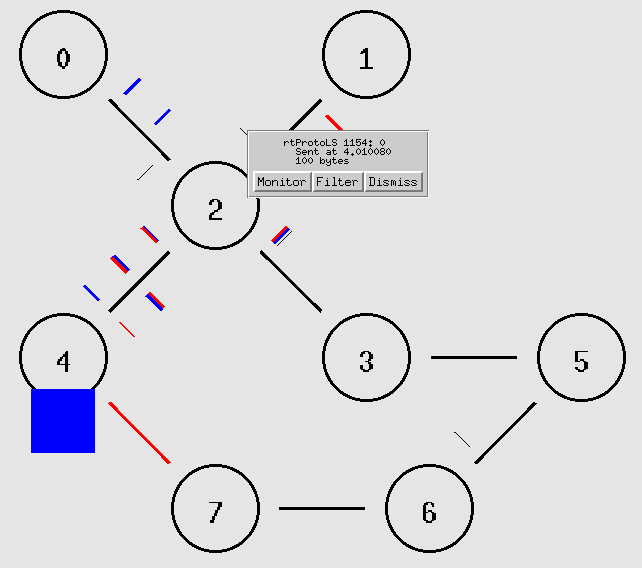
\includegraphics[width=0.9\textwidth]{assets/tp2/envoiInfoRuptureAuxautresLS.png}
        \caption{Mise a jour des autres nœuds LS}
        \label{infoAutres}
    \end{minipage}
\end{figure}



Dans ce protocole, lors de la rupture de lien entre le nœud 4 et 7, plusieurs paquets sont envoyés. Tout d'abord par le nœud 4 au nœud 2, mais aussi le nœud 7 au nœud 6 comme nous le montre la figure \ref{ruptureLS}. Après cela ces nœuds vont à leurs tours informer les autres de la rupture pour qu'ils puissent mettre à jour leurs table de routage, voir figure \ref{infoAutres}. On peut aussi remarquer que vu tous les nœuds ont une connaissance globale du réseau, le nœud 4 après la détection de la rupture va stocker les nouveau paquets reçu, calculer un nouveau chemin et les envoyer sur la nouvelle route, ici le nœud 4 renvoie les paquets au nœud 2. Seul les paquets qui se trouvaient sur le lien seront perdu. Comme nous pouvant le voir dans le figure \ref{detectRuptureLS}, la détection de rupture s’est effectuée au bout de 0.01s.


\begin{figure}[H]
	\begin{center}
		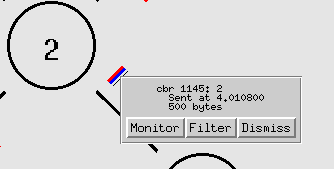
\includegraphics[width=0.5\textwidth]{assets/tp2/DetecterRuptureLS.png}
	\end{center}
	\caption{Détection de la rupture de lien LS}
	\label{detectRuptureLS}
\end{figure}


A t=5.0s le lien entre les nœuds 4 et 7 a été rétablit et redevient donc le meilleur chemin, avec le protocole à vecteur distance le rétablissement a été détecté en 0.010006s voir figure \ref{retDV} et pour le protocole à état de lien en 0.01008s voir figure \ref{retLS}.

\begin{figure}[H]
    \begin{minipage}[c]{.5\linewidth}
        \centering
        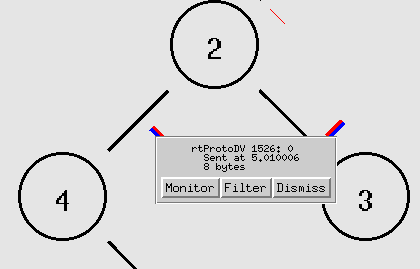
\includegraphics[width=0.9\textwidth]{assets/tp2/retablissementlienDV.png}
        \caption{Détection rétablissement DV}
        \label{retDV}
    \end{minipage}
      \hfill%
    \begin{minipage}[c]{.5\linewidth}
        \centering
        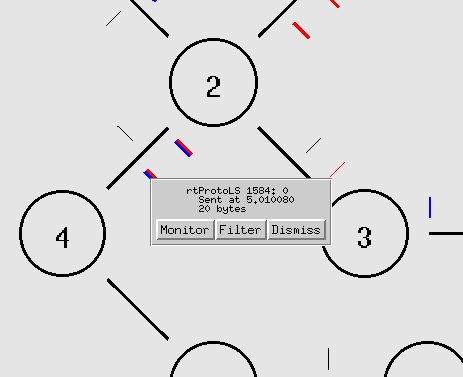
\includegraphics[width=0.9\textwidth]{assets/tp2/retablissementLienLS.png}
        \caption{Détection rétablissement LS}
        \label{retLS}
    \end{minipage}
\end{figure}

Lors de cet exercice, nous avons pu remarquer qu’il existe différents types de mise à jour des tables de routage qui sont au nombre de trois. Nous allons les présenter ci-dessous :

\begin{itemize}
	\item \textbf{Mise à jour initiale} : la toute première mise à jour qui s’effectue avant même d’envoyer les premiers paquets, voir figures \ref{initDV} et \ref{initLS}
	\item \textbf{Mise à jour déclenchée} : mise à jour des tables de routage lorsqu’il y a détection de rupture d’un des liens, voir figures \ref{ruptureDV} et \ref{ruptureLS}.
	\item \textbf{Mise à jour ponctuelle} : mise à jour qui s’effectue qui s’effectue ponctuellement tous les deltas t. Dans notre simulation (en protocole de routage à vecteur distance seulement) la mise à jour ponctuelle s’effectue toutes les 2s voir figure \ref{misePeriodique}.
	
Cette mise a jour dans le protocoles à état de lien permet de mettre a jour la table de routage des voisins. Par exemple le nœud 2 va envoyer au nœud 4 sa table de routage dans lequel il dit qu'il peut aller vers les nœuds 0, 1, 3, 5, 6, 7 avec un certain coût, le nœud 4 va alors voir si les informations passé par le nœud 4 améliorent certain entrés de sa table de routage, si c'est le cas alors il va faire confiance au nœud 2 et va mettre a jour sa table. Donc si plus tard le nœud 7 veux envoyer un paquet au nœud 0, il sait avec sa table de routage que s'il veux atteindre le nœud 0 il faut qu'il envoie au nœud 4 qui se débrouille d'acheminer le paquet. Le nœud 4 va aussi regarder dans sa table de routage et va voir que pour aller vers le nœud 0 il faut l'envoyer au nœud 2, et le nœud vu qu'il est directement relié au nœud 0 va directement transmettre le paquet.
\end{itemize}

\begin{figure}[H]
	\begin{center}
		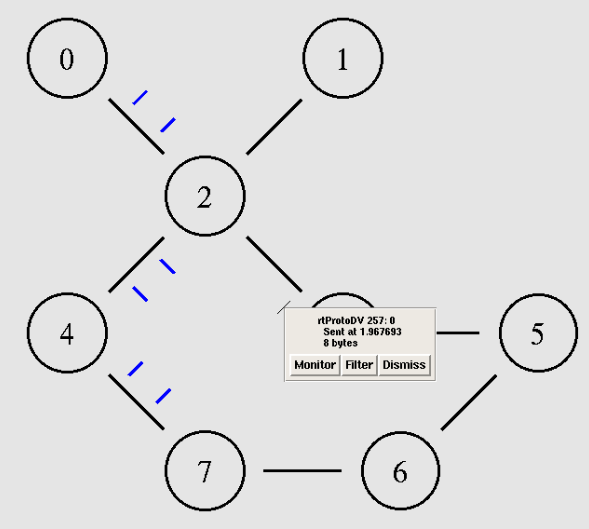
\includegraphics[width=0.5\textwidth]{assets/tp2/miseAjourPeriodiqueDV.png}
	\end{center}
	\caption{Mise a jour périodique DV}
	\label{misePeriodique}
\end{figure}

Pour résumer ce que nous avons pu voir dans cet exercice nous présentons nos analyses sous la forme du tableau comparatif ci-dessous :

\noindent
\begin{tabular}{|R{4cm}|M{5cm}|M{5cm}| }
    \hline
     					   & 
     	Vecteur Distance  &  
     	Etat de Liens 
 	\tabularnewline
    \hline
     	Mises à jour de routage & 
     	\begin{itemize}
     		\item Initiale
     		\item Déclenchée
     		\item Ponctuelle
		\end{itemize}  & 
		\begin{itemize}
			\item Initiale
			\item Déclenchée
		\end{itemize}	   
	\tabularnewline
    
    \hline 
    	Détection de la rupture & 
    	0.3s & 
    	0.01s 
    \tabularnewline
  
   	\hline 
   		Détection du rétablissement & 
   		0.01s & 
   		0.0108s 
   	\tabularnewline
   	
   	\hline 
   		Convergence &
   	 	Lente  & 
   	 	Rapide 
   	\tabularnewline
   	
   	\hline 
   		Comportement du nœud 4 à la rupture & 
   		Le nœud drop tous les paquets qui lui parviennent s’il ne trouve pas le nœud suivant. & 
   		Le nœud recalcule un nouveau chemin et redirige vers le nœud 2 tous les paquets qui lui parviennent. 
   	\tabularnewline
   	
   	\hline 
   		Paquets perdus  & 
   		Tous les paquets reçus entre la rupture et le moment ou l’émetteur retrouve un nouveau chemin. &
   		Seulement les paquets qui étaient sur le lien lors de la rupture. 
   	\tabularnewline
   	
   	\hline
\end{tabular}







\subsection{Exercice 2: Routage et contrôle de congestion TCP}

Dans cette partie du TP nous allons devoir simuler un réseau et observer et comprendre l’évolution de la taille de la fenêtre d’un flux TCP en fonction du RTT (Round Type Time). Le script complet est disponoble dans l'annexe \ref{tp2Exo2}, nous détailleront ici que les nouvelles commandes.\\


Pour la réalisation du réseau souhaité il nous a fallu utiliser des commandes déjà présentées précédemment ainsi que deux nouveautés :

\textbf{Renommer un nœud} :Pour renommer le nom des nœuds par des lettres avec les commandes suivantes :

\begin{lstlisting}[language=tcl, numbers=none, framexleftmargin=0pt, 	framextopmargin=0pt, framexbottommargin=0pt]
$A label "A"
$B label "B"
$C label "C"
$D label "D"
\end{lstlisting}

\textbf{Changement des formes source et destination} : Cette commande change le cercle habituel représentant le nœud en hexagone.
\begin{lstlisting}[language=tcl, numbers=none, framexleftmargin=0pt, 	framextopmargin=0pt, framexbottommargin=0pt]
#changement des formes source et destination
$A shape hexagon
$D shape hexagon
\end{lstlisting}

Pour aussi visualiser la taille de la fenetre TCP nous avons aussi ajouter cette partie du code pour pouvoir tracer le graph a l'aide de xgraph.

\begin{lstlisting}[language=tcl, numbers=none, framexleftmargin=0pt, 	framextopmargin=0pt, framexbottommargin=0pt]
# CTP WINDOW SIZE
# Pour pouvoir visualiser la taille de la fenetre TCP a l'aide de xgraph
set f_window [open tcpWindow.tr w]

proc plot_tcp {} {
    global f_window tcp ns
    if { [$tcp set cwnd_] < [$tcp set window_] } {
        puts $f_window "[$ns now] [$tcp set cwnd_]"
    } else {
        puts $f_window "[$ns now] [$tcp set window_]"
    }
$ns at [expr [$ns now] + 0.1] plot_tcp

}
$ns at 0.01 "plot_tcp"
\end{lstlisting}

Ici on ouvre un fichier en écriture appelé \textit{fwindow}. Puis on crée une procédure appelé \textit{plotTcp} qui va être appelé tout les 0.1s. A chaque appelle de la procédure on regarde le minimum entre les attribut de la l'instance TCP avec la variable \$tcp, on regarde le minimum entre cwnd et le window et on écrit dans le fichier le temps actuel et soit le cwnd soit le window. A la fin nous obtenant un graph figure \ref{graphXgraph} mais en abscisse on obtient le temps au lieu du RTT, c'est pour cela que nous avons refait un nouveau graph figure \ref{graphExcel} avec un tableur avec cette fois le RTT en abscisse.

Grâce à notre code, nous obtenons le réseau suivant figure \ref{miseAjourRoutageTCPDV}, nous pouvons y voir les premiers échanges de tables de routages (mise à jour initiale). Puis il y a établissement de la connexion entre l’émetteur et le récepteur.


\begin{figure}[H]
	\begin{center}
		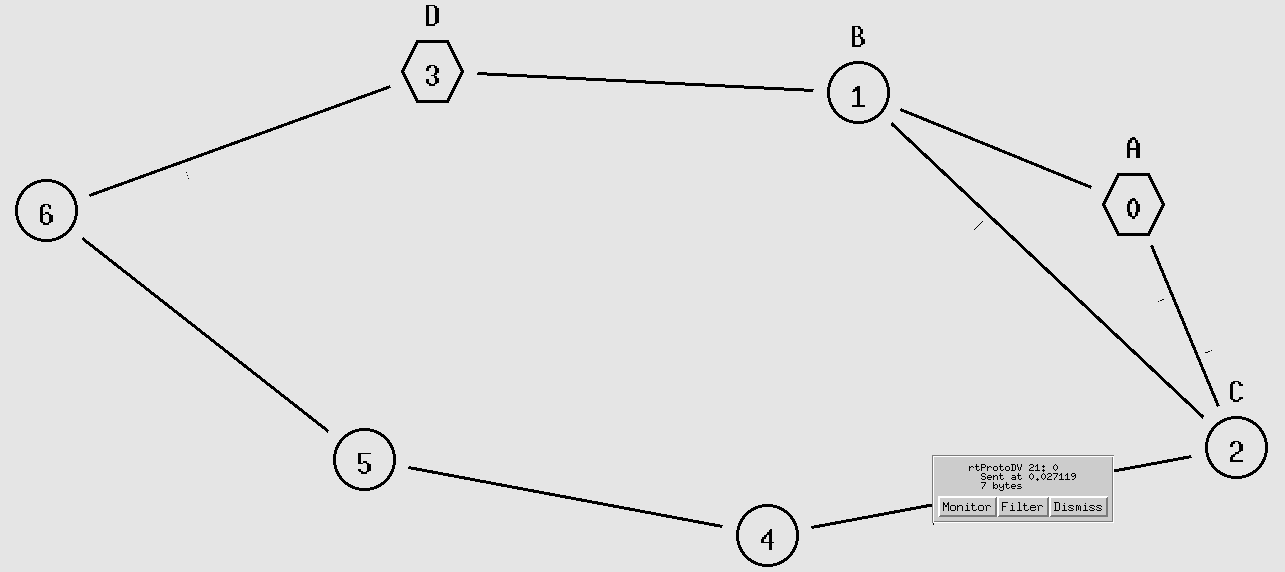
\includegraphics[width=0.5\textwidth]{assets/tp2/miseAjourRoutage.png}
	\end{center}
	\caption{Initialisation des tables de routage}
	\label{miseAjourRoutageTCPDV}
\end{figure}

Lors du premier envoie de paquet, l’émetteur envoie deux paquets comme nous pouvons le voir sur la figure \ref{premPaquet}

\begin{figure}[H]
	\begin{center}
		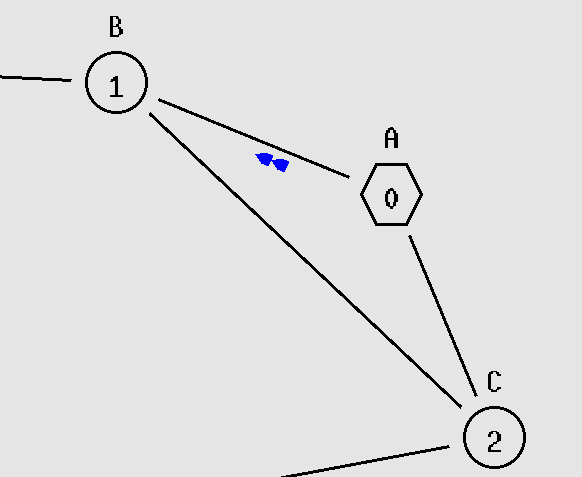
\includegraphics[width=0.5\textwidth]{assets/tp2/premierEvoiepaquet.png}
	\end{center}
	\caption{Premiers paquets envoyés}
	\label{premPaquet}
\end{figure}


Lors du démarrage d'une connexion, tcp ne connaissons pas le lien qu'il y a entre lui et le destinataire, donc il va progressivement augmenter le nombre de paquets qu'il envoie. Le but est donc de trouver la bande passante disponible, et utiliser toutes les ressources à disposition, en s'adaptant au capacité du réseau (contrôle de congestion) avec la méthode \textbf{slow start}. Le nombre de doublera à chaque envoie après confirmation de la réception des paquets précédents. Au bout d'un moment le nombre de paquet deviens constant,égale a 20 voir figure \ref{envoie20}. Ici on peut supposer que 2O le rwnd (receiver window), que l'émetteur et le récepteur ont choisie au moment de l’établissement de la connexion. La tcp s'adapte au capacité du récepteur (contrôle de flux).

\begin{figure}[H]
	\begin{center}
		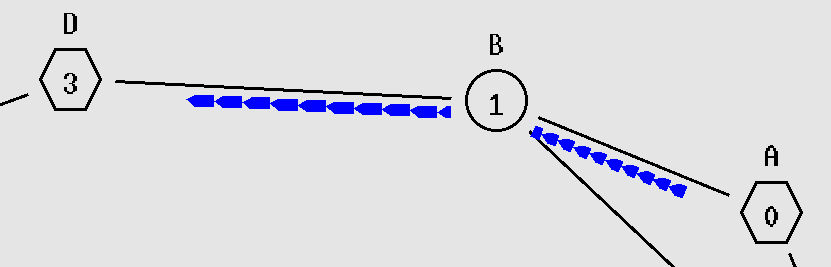
\includegraphics[width=0.5\textwidth]{assets/tp2/envoie20paquet.png}
	\end{center}
	\caption{Envoie de 20 paquet}
	\label{envoie20}
\end{figure}


Suite à cette rupture de lien, figure \ref{rupturelienT}, il a une mise à jour déclenchée qui s’effectue puis les paquets vont prendre un nouveau chemin en passant par le nœud C voir figure \ref{nouveauchemain}. On peut aussi voir que après la rupture l’émetteur n'envoie qu'un paquet, cela est du a la détection de perte de paquet avec le mécanisme de timeout.

\begin{figure}[H]
	\begin{center}
		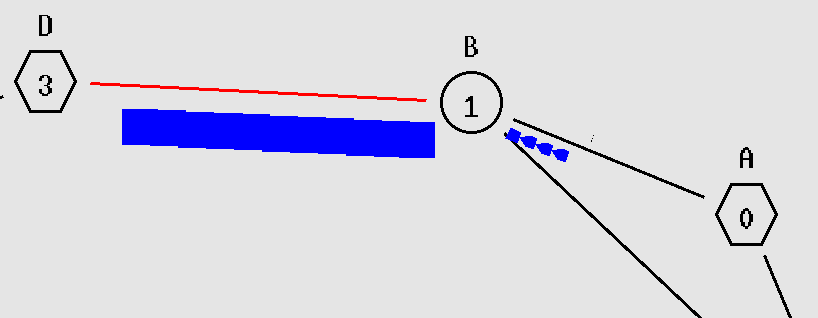
\includegraphics[width=0.5\textwidth]{assets/tp2/ruptureLien.png}
	\end{center}
	\caption{Rupture de lien}
	\label{rupturelienT}
\end{figure}

\begin{figure}[H]
	\begin{center}
		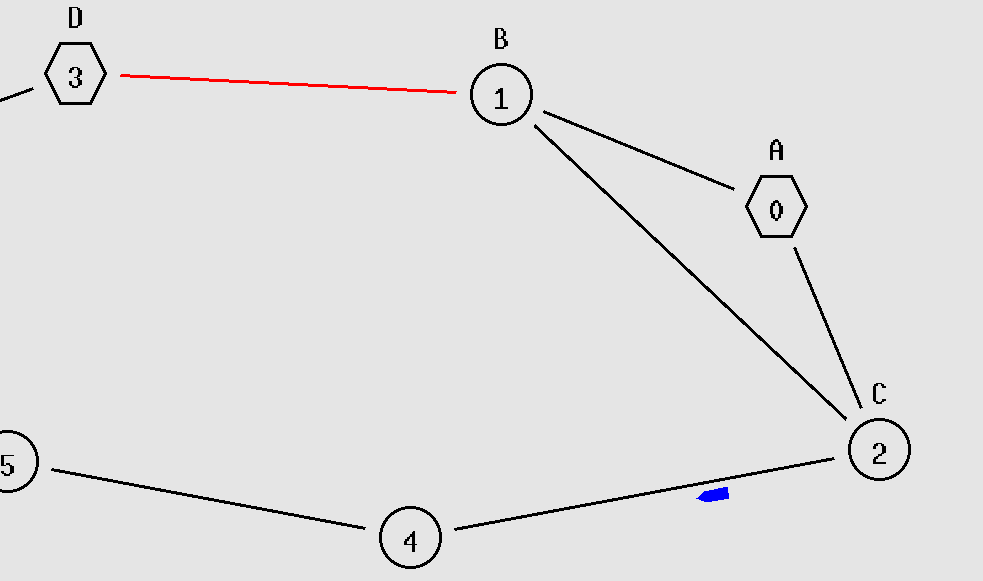
\includegraphics[width=0.5\textwidth]{assets/tp2/Nouveauchemain.png}
	\end{center}
	\caption{Comportement après rupture de lien}
	\label{nouveauchemain}
\end{figure}

Par la suite, le lien rompu va à nouveau être actif et le flux de paquet va à nouveau reprendre son chemin en passant par le nœud B après avoir fait une mise à jour de la table de routage et recalculé le meilleur chemin.\\


Pour pouvoir mieux comprendre les mécanismes de TCP, on a réalisé 2 graphiques disponible dans la figure \ref{graphXgraph} et \ref{graphExcel}, un généré avec le script et visualisé avec xgraph et l'autre fait avec un tableur. Pour analyser les résultats nous alors utiliser le graphique \ref{graphExcel}.\\


Nous allons analyser les résultats obtenus sur ce graphique \ref{graphExcel}. Tous d’abord nous pouvons remarquer, que dans un premier temps l’émetteur effectue un slow start (l’émetteur double à chaque fois le nombre de paquet qu’il envoi). Cette phase est un contrôle de congestion. Arrivé, à 20 paquets la fenêtre n’augmente plus ceci est dû au récepteur qui a une fenêtre de réception de 20 paquets c’est ici un contrôle de flux qui s’effectue.

Ensuite, il y a la rupture de lien à cause de laquelle des paquets sont perdus. A cause de ces
pertes, l’émetteur va ré-effectuer un contrôle de congestion mais cette fois ci en deux
temps :
\begin{itemize}
	\item Dans un premier temps, l’émetteur fait un slow start en démarrant avec l’envoi d’un seul paquet jusqu’à dix paquets. Ces valeurs ne sont pas dues au hasard mais suite à une perte il est normale de repartir avec un seul paquet et la valeur dix est obtenu car c’est la division par deux de la dernière taille de fenêtre accusée normalement (ici vingt).

	\item Dans un second temps, l’émetteur effectue un congestion avoidance c’est-à- dire qu’il augmente la taille de la fenêtre en ajoutant un paquet à la fois.
\end{itemize}

Le contrôle de congestion va se terminer lorsque la taille de la fenêtre va atteindre vingt paquets puisque c’est le contrôle de flux qui prendre la relève en maintenant la taille d’envoi à vingt pour ne pas dépasser la taille de ce que peut recevoir le récepteur.\\

\noindent
Perte de segments TCP :

Dans notre cas, la perte de segment a été générée par la rupture d’un lien entre deux nœuds mais il est envisageable que dans d’autre cas cette perte soit due à différents scénarios comme ceux-ci :
\begin{itemize}
	\item Un TTL (Time To Live) trop court qui empêche le paquet d’arriver à destination -$>$ Dans ce cas il y a envoie d'un message ICMP
	\item Pas de chemin possible pour atteindre le récepteur -$>$ Envoie d'un message ICMP
\end{itemize}
 

\begin{figure}[H]
	\begin{center}
		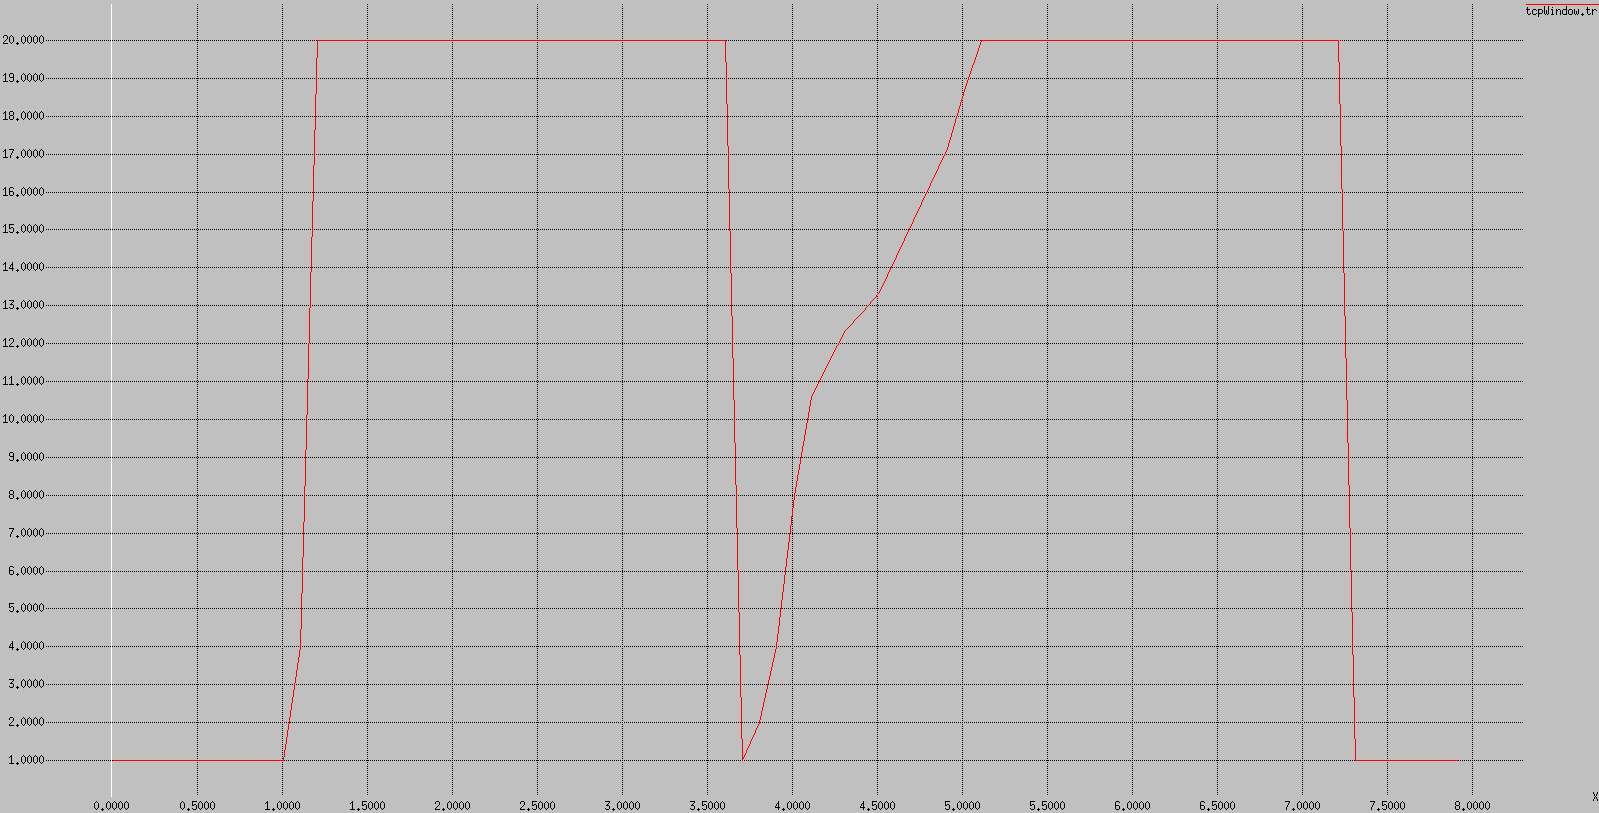
\includegraphics[width=1\textwidth]{assets/tp2/tcpWindowXgraph.png}
	\end{center}
	\caption{Évolution de la fenêtre TCP en fonction du RTT avec xgraph}
	\label{graphXgraph}
\end{figure}

\begin{landscape}
\begin{figure}[H]
	\begin{center}
		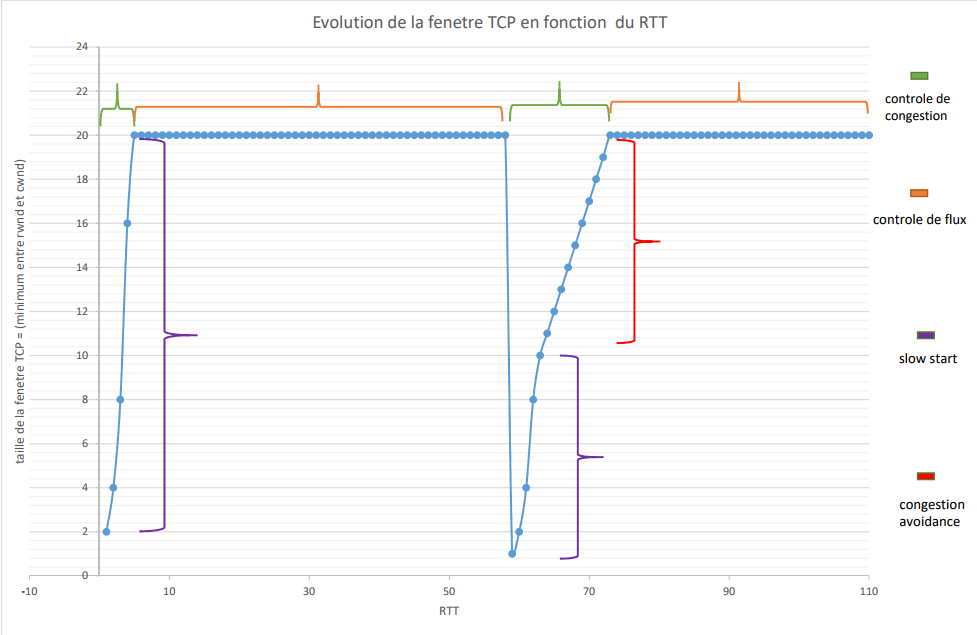
\includegraphics[width=1.3\textwidth]{assets/tp2/graphiqueExcel.png}
	\end{center}
	\caption{Évolution de la fenêtre TCP en fonction du RTT}
	\label{graphExcel}
\end{figure}
\end{landscape}



Ce TP nous a permis de voir les différences entre un protocole à vecteur distance et un protocole à état de liens, comprendre comment réagit le réseau lorsqu’il y a une rupture de lien entre deux nœuds. La seconde partie du TP nous a quant à elle permit de visualiser comment l’émetteur adapte la taille de sa fenêtre d’envoie en fonction de différents éléments comme la congestion du réseau, une perte de paquet et la taille de la fenêtre du récepteur.




\pagebreak
% Partie 3
\section{TP 3: Utilisation de xgraph et NS-2 pour visualiser les performances d'un réseau}
Dans ce dernier tp nous allons utiliser xgraph avec ns2 pour pouvoir visualiser les performances d'un réseau donné. 

Le script complet est disponible dans l'annexe \ref{tp3Exo1} avec les commentaires 

\subsection{Visualisation du réseau avec nam}
Après avoir modifié le script on peut visualiser le réseau a l'aide de nam. La figure \ref{startTp3} représente le réseau en action.

\begin{figure}[H]
	\begin{center}
		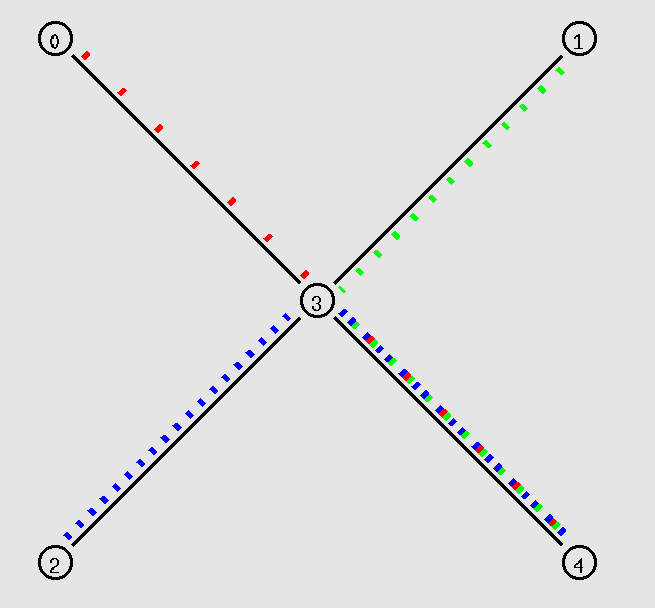
\includegraphics[width=0.5\textwidth]{assets/tp3/tp3Start.png}
	\end{center}
	\caption{Simulation du réseau}
	\label{startTp3}
\end{figure}


Autour des 10s la source 2 commence a emmètre comme le montre la figure \ref{demarageSource2}

\begin{figure}[H]
	\begin{center}
		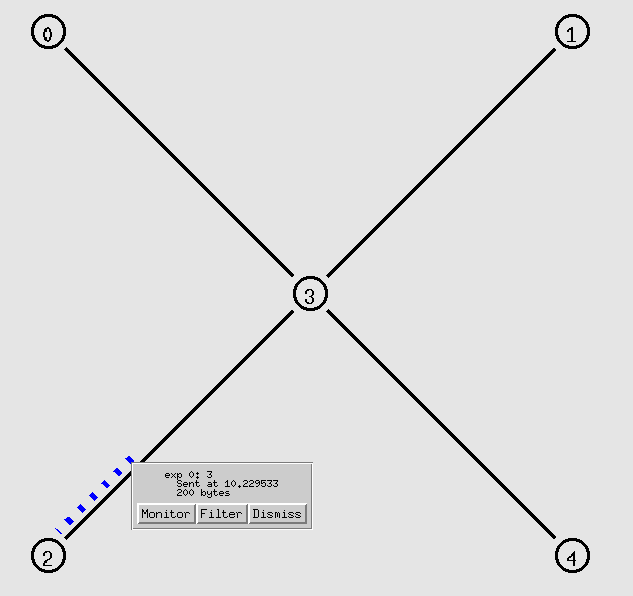
\includegraphics[width=0.5\textwidth]{assets/tp3/demarageSource2.png}
	\end{center}
	\caption{Démarrage de la source 2}
	\label{demarageSource2}
\end{figure}


Ensuite un peut plus tard c'est la source 0 qui démarre comme on peut le voir dans la figure \ref{demarageSource0}

\begin{figure}[H]
	\begin{center}
		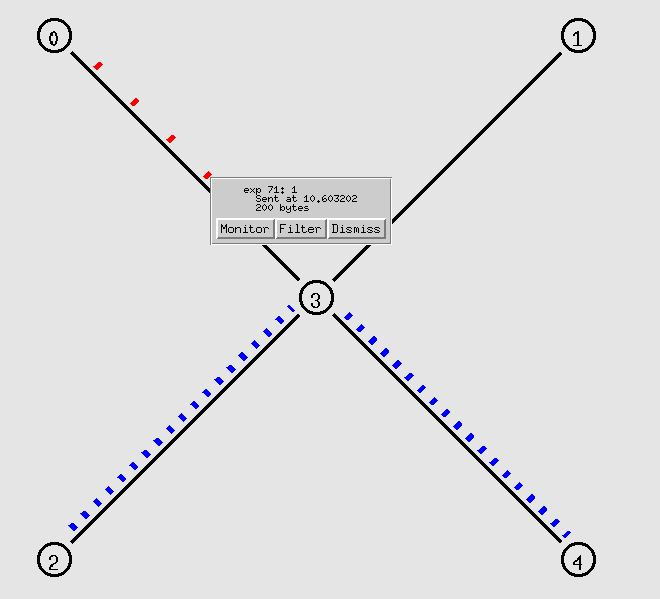
\includegraphics[width=0.5\textwidth]{assets/tp3/demarageSource0.png}
	\end{center}
	\caption{Démarrage de la source 0}
	\label{demarageSource0}
\end{figure}

Pour finir c'est la source 1 qui démarre l’émission, illustré par la figure \ref{demarageSource1}

\begin{figure}[H]
	\begin{center}
		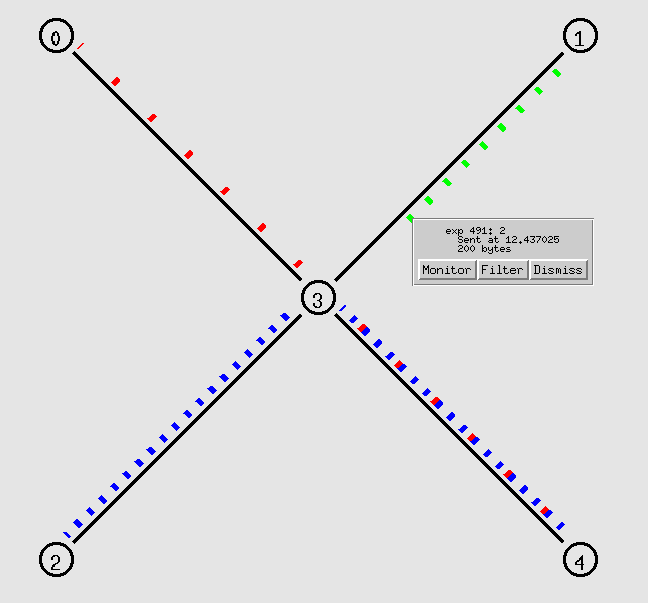
\includegraphics[width=0.5\textwidth]{assets/tp3/demarageSource1.png}
	\end{center}
	\caption{Démarrage de la source 1}
	\label{demarageSource1}
\end{figure}

Pendant un certain temps les trois sources émettent en même temps. Au bout d'un certain temps elles vont arrêter l’émission indépendamment les unes des autres ( dans la figure \ref{finBurstSource2} on peut voir un exemple pour la source 2) puis reprendre plus tard comme le montre la figure \ref{repriseBurstSource2}.

Les autres sources partagent également cette  particularité qui est due à l'utilisation d'un trafic de type \textbf{exponential}. Ils émettent en mode burst c'est à dire qu'ils envoie des données pendant un certain temps puis arrêtent l'émission puis la reprennent plus tard. Ces paramètres sont configurés dans le script en changement les attribut (rate, burstTime, idleTime) de la classe Exponential.
 
\begin{figure}[H]
	\begin{center}
		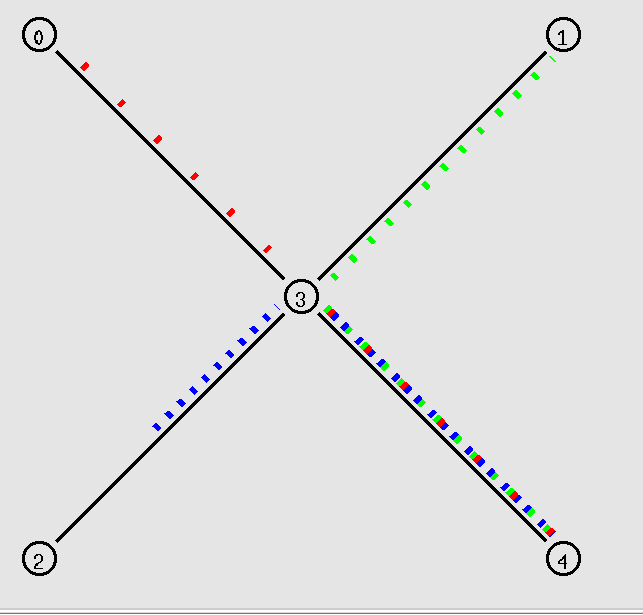
\includegraphics[width=0.5\textwidth]{assets/tp3/finduBurstSource2.png}
	\end{center}
	\caption{Fin d'émission de la source2}
	\label{finBurstSource2}
\end{figure}

\begin{figure}[H]
	\begin{center}
		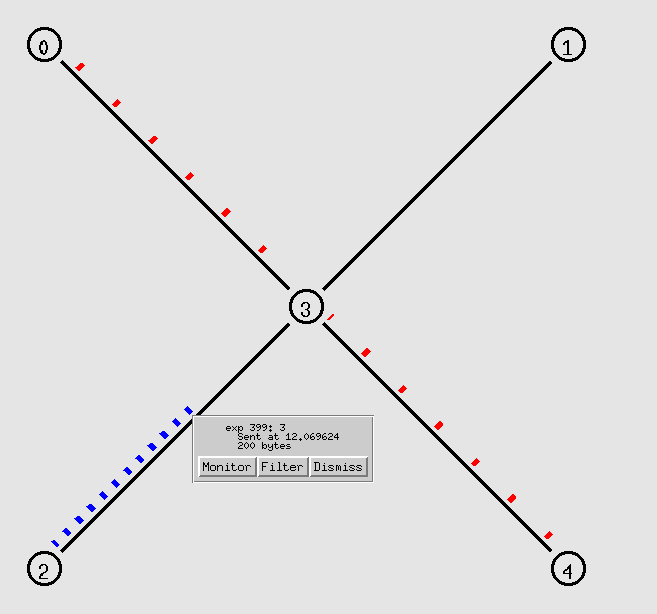
\includegraphics[width=0.5\textwidth]{assets/tp3/repirseDuBurstSource2.png}
	\end{center}
	\caption{Reprise de l'émission pour la source2}
	\label{repriseBurstSource2}
\end{figure}

\subsection{Étude détaillé des procédures}
Dans cette partie nous allons expliquer en détaille les deux procédures attach-expo-traffic et record

Voici le code commenté pour la procédure attach-expo-traffic

\begin{lstlisting}[language=tcl,  numbers=none, framexleftmargin=0pt, 	framextopmargin=0pt, framexbottommargin=0pt], label={tp1Exo1}, caption={Procédure Attach-expo-traffic}]
#Procédure pour associer un trafic à a une source et retourne le traffic
#@param:
#	node: le noeud source
#	sink: l'agent qui devra recevoir les données
#	size: la taille des paquets
#	burst: temps moyen de fonctionnement du générateur
#	idle: temps d'arrêt moyen du générateur
#	rate: taux d'envoi pendant fonctionnement
#	color: couleur du paquet
#@return : le trafic crée
proc attach-expoo-traffic { node sink size burst idle rate color } { 
	# Créer une instance de Simulator
	set ns [Simulator instance]
	
	#Créer une source UDP et l'attacher au noeud passé en paramètre
	set source [new Agent/UDP]
	$ns attach-agent $node $source
	
	#Céer un traffic Exponential et modifier ses attributs
	set traffic [new Application/Traffic/Exponential]
	$traffic set packetSize_ $size
	$traffic set burst_time_ $burst
	$traffic set idle_time_ $idle
	$traffic set rate_ $rate

	#Attacher le trafic a la source et connecter la source a l'agent qui va recevoir les données
	$traffic attach-agent $source
	$ns connect $source $sink

	#colorier le flux
	$source set class_ $color

	return $traffic
}
\end{lstlisting} 

~\\
La procédure attach-expoo-traffic, contient sept paramètres (six qui  étaient présents et une \textit{color} ajouté pour modifier la couleur du trafic)  :
\begin{itemize}
	\item node : nœud source
	\item sink : l'agent qui devra recevoir les données (ici un agent de type LossMonitor)
	\item size : taille des paquets qui seront générés
	\item burst : temps moyen de fonctionnement du générateur
	\item idle : temps d'arrêt moyen du générateur
	\item rate : taux d'envoi pendant fonctionnement (débit d'émission)
	\item color: couleur du paquet
\end{itemize}
 
La procédure va créer une instance de Simulator, créer un agent UDP et l'attacher au nœud passé en paramètre, ensuite elle va créer une nouvelle instance de type Exponential et changer ses attributs avec ceux passé en paramètre, puis elle va attacher le trafic a la source et connecter la source avec l'agent qui va recevoir les données. Pour finir, elle colorie le flux de la source avec la couleur en paramètre et retourne l'instance trafic crée.\\

Le code ci-dessus représente la fonction record avec les commentaires
\begin{lstlisting}[language=tcl,  numbers=none, framexleftmargin=0pt, 	framextopmargin=0pt, framexbottommargin=0pt], label={tp1Exo1}, caption={Procédure record}]
#Procédure qui enregistre les données
proc record {} {
	global sink0 sink1 sink2 f0 f1 f2

	set ns [Simulator instance]
	
	set time 0.5
	#Récuperer les octets recus par les diffèrent trafic sink
	set bw0 [$sink0 set bytes_]
	set bw1 [$sink1 set bytes_]
	set bw2 [$sink2 set bytes_]
	set now [$ns now]
	
	#Écrire dans les fichiers
	puts $f0 "$now [expr $bw0/$time*8/1000000]"
	puts $f1 "$now [expr $bw1/$time*8/1000000]"
	puts $f2 "$now [expr $bw2/$time*8/1000000]"
	
	#Remetre les valeurs a 0
	$sink0 set bytes_ 0
	$sink1 set bytes_ 0
	$sink2 set bytes_ 0
	
	#Rappeler la procedure apres un temps donnée
	$ns at [expr $now+$time] "record"
}
\end{lstlisting} 

Dans un premier temps cette procédure va récupération des variables globales telos que sink0 sink1 sink2 f0 f1 f2, affecter l'instance de Simulator, définir une variable \textbf{time} qui servira a déterminer au bout de combien de temps on rappelle la procédure. Dans un second temps, elle récupère  dans bwx le nombre d'octets reçu par le trafic x, puis récupère a l'aide de l'instance de Simulator le temps d’exécution actuel. Ensuit elle va écrire dans les différents fichier le temps actuel et le nombre d'octets reçu en MB/s. Et pour finir remise à zéro des attributs sink pour pouvoir mesurer la nouvelle quantité d’octets envoyés depuis la dernière mesure la prochaine fois qu'on revient dans la procédure. Avant de quitter la procédure on définit un nouveau timer a lequel on doit appeler la fonction record, ici on prend le temps actuel et on ajoute la variable time définit plus haut


\subsection{Étude des différents courbes}

\begin{figure}[H]
	\begin{center}
		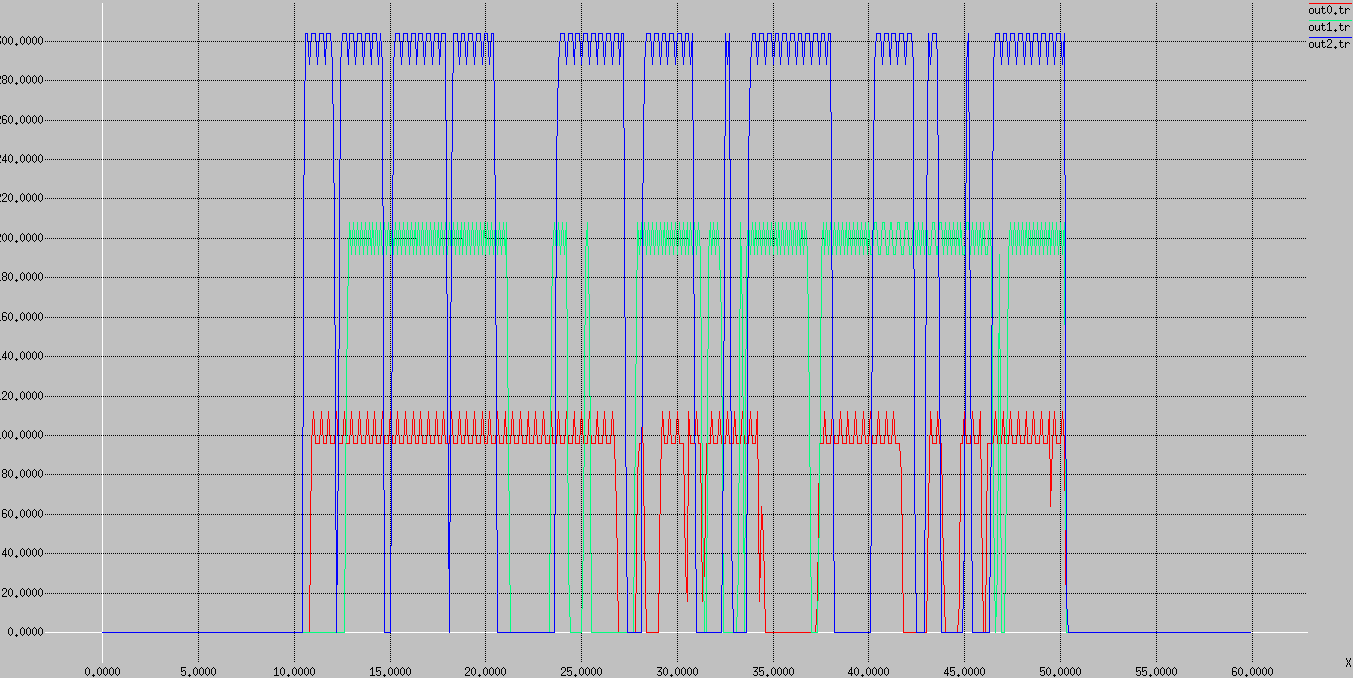
\includegraphics[width=0.9\textwidth]{assets/tp3/xgraph01s.png}
	\end{center}
	\caption{Courbe xgraph avec un temps d'enregistrement de 0.1s}
	\label{xgrap01s}
\end{figure}

\begin{figure}[H]
	\begin{center}
		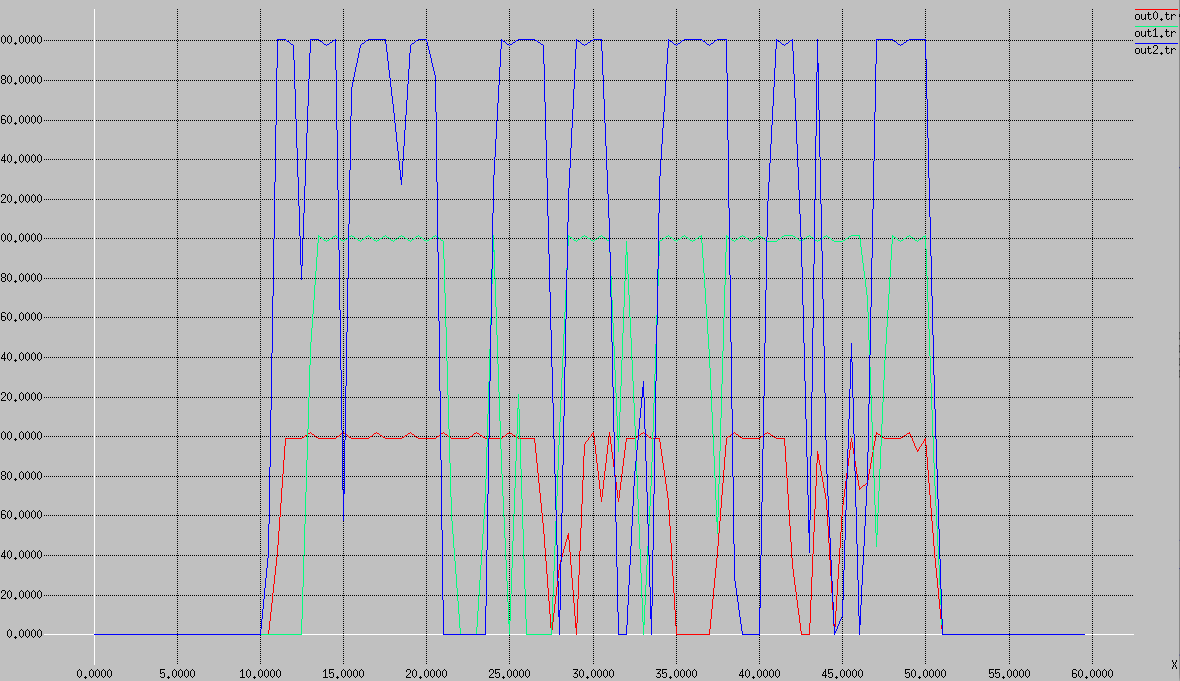
\includegraphics[width=0.9\textwidth]{assets/tp3/xgraph05s.png}
	\end{center}
	\caption{Courbe xgraph avec un temps d'enregistrement de 0.5s}
	\label{xgraph05s}
\end{figure}

\begin{figure}[H]
	\begin{center}
		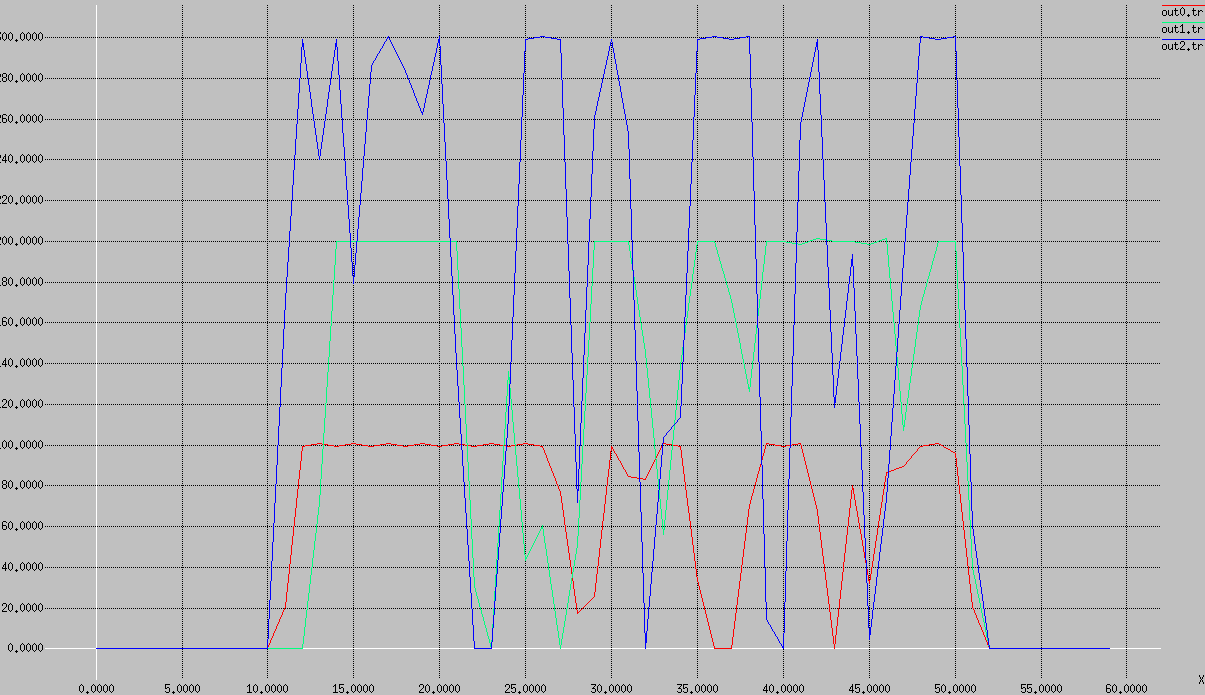
\includegraphics[width=0.9\textwidth]{assets/tp3/xgraph1s.png}
	\end{center}
	\caption{Courbe xgraph avec un temps d'enregistrement de 1s}
	\label{xgraph1S}
\end{figure}

En comparent les figures \ref{xgrap01s}, \ref{xgraph05s}, \ref{xgraph1S} on remarque que plus le temps d’actualisation est élevé (c'est a dire plus la variable \textit{time} est petite), plus on a de points sur la courbe et plus la précision augmente, ce qui augmente la détection des retours à zéro. On peut voir dans la figure \ref{xgraph1S} à 15 secondes un retour à zero alors que dans les courbes \ref{xgrap01s} et \ref{xgraph05s} le retour à 0 n'est pas présent, et même dans la figure \ref{xgraph1S} on pourrait pense que le trafic ne s'est pas arrêter vers les 15sec alors cela s'est produit dans notre réseau. Un retour a zero sur la courbe représente l’arrêt d'émission du trafic \\


~\\
\\
\\
\\
\\


Pour conclure ce dernier tp, nous avons vu comment se servir de xgraph afin de visualiser les performances d'un réseau, de plus on s'est plus familiariser avec le langage OTcl. Avec l'analyse des courbes nous avons aussi vu que était nécessaire de tracer une courbe avec un temps d’actualisation très cours pour mieux visualiser et se rapprocher au plus du comportement du réseau simulé.



\pagebreak
\section*{Conclusion}
\addcontentsline{toc}{section}{Conclusion}
Pour conclure, au cours de ces TP nous avons pris en main le logiciel NS2 qui permet la simulation de réseaux. A l'aide de celui-ci nous avons pu appréhender et comprendre comment réagi un reseau lors de différentes situation. Nous avons vu les différents types de protocoles de routage et leurs spécificités mais également comment s'effectue un contrôle de congestion et un contrôle de flux.

D'un point de vu personnel, nous avons trouvé que ces TP sont une excellente manière d'aider à l'entière compréhension du cours. Le fait d'illustrer ce que l'ont voit lors des cours est bénéfique permet de mieux comprendre retenir les choses.

\pagebreak
\section*{Annexes}
\addcontentsline{toc}{section}{Annexes}

\begin{enumerate}
	
	\item \textbf{Script du TP1 - Exercice 1}

\begin{lstlisting}[language=tcl, label={tp1Exo1}, caption={TP1 - Exercice1}]
#Création d'une instance de l'objet Simulator
set ns [new Simulator]

#Ouvrir le fichier trace pour nam
set nf [open out.nam w]
$ns namtrace-all $nf

#Définir la procedure de terminaison de la simuatation
proc finish {} {
	global ns nf
	$ns flush-trace
	#fermer le fichier trace
	close $nf
	#Exectuer le nam avec en entrée le fichier trace
	exec nam out.nam &
	exit 0
}

#Insérer votre code
set NodeNb 2
for {set i 0} {$i<$NodeNb} {set i [expr $i+1]} {set n($i) [$ns node]}
#connecter les deux noeuds
$ns duplex-link $n(0) $n(1) 1Mb 10ms DropTail
set udp [new Agent/UDP]
#atacher l'aplication udp au noeud 0
$ns attach-agent $n(0) $udp 
#creattion d'un source de trafique
set cbr [new Application/Traffic/CBR]
$cbr set packetSize_ 500bytes
$cbr set interval_ 0.005s
#connecter le cbr a l'agent UDP
$cbr attach-agent $udp

#creation de l'agent null
set agentNull [new Agent/Null]
#atacher l'agent null au noeud 1
$ns attach-agent $n(1) $agentNull 
#connecter l'agent null et l'agent udp
$ns connect $udp $agentNull 
#declancher le trafic cbf
$ns at 1 "$cbr start"
$ns at 4.5 "$cbr stop"

#Appeler la procédure de terminaison apres un temmps t 
$ns at 5.0 "finish"

#Executer la simulation
$ns run
\end{lstlisting} 

~\\

\item \textbf{Script du TP1 - Exercice 2}
\begin{lstlisting}[language=tcl, label={tp1Exo2}, caption={TP1 - Exercice2}]
#Création d'une instance de l'objet Simulator
set ns [new Simulator]

#Ouvrir le fichier trace pour nam
set nf [open out2.nam w]
$ns namtrace-all $nf

#Définir la procédure de terminaison de la simulation
proc finish {} {
	global ns nf
	$ns flush-trace
	#fermer le fichier trace
	close $nf
	#Exectuer le nam avec en entrée le fichier trace
	exec nam out2.nam &
	exit 0
}

#Insérer votre code
set NodeNb 4
for {set i 0} {$i<$NodeNb} {set i [expr $i+1]} {set n($i) [$ns node]}

#connecter les deux noeuds
$ns duplex-link $n(0) $n(2) 2Mb 10ms DropTail
$ns duplex-link $n(1) $n(2) 2Mb 10ms DropTail
$ns duplex-link $n(2) $n(3) 1.7Mb 20ms DropTail

#creation des agents
set tcp [new Agent/TCP]
set udp [new Agent/UDP]
set agentNull [new Agent/Null]
set tcpSink [new Agent/TCPSink] 

#creation des applications
set ftp [new Application/FTP]
set cbr [new Application/Traffic/CBR]

#attacher agent aux noeuds
$ns attach-agent $n(0) $tcp
$ns attach-agent $n(1) $udp
$ns attach-agent $n(3) $tcpSink
$ns attach-agent $n(3) $agentNull

#connecter les applications aux agents 
$cbr attach-agent $udp
$ftp attach-agent $tcp

#connecter les agents avec les agents coresspondant
$ns connect $udp $agentNull 
$ns connect $tcp $tcpSink 

#configurations 
$ns queue-limit $n(2) $n(3) 10

$cbr set packetSize_ 1000bytes
$cbr set rate_ 1Mb

$ns duplex-link-op $n(0) $n(2) orient right-down
$ns duplex-link-op $n(1) $n(2) orient right-up
$ns duplex-link-op $n(2) $n(3) orient right

#coloration
$ns color 1 Red
$ns color 2 Blue
$ns color 3 Green

$tcp set class_ 1
$udp set class_ 2
#$tcpSink set class_ 3

#declancher le trafic cbf
$ns at 0.1 "$cbr start"
$ns at 4.5 "$cbr stop"
#declancher le trafic ftp
$ns at 1 "$ftp start"
$ns at 4 "$ftp stop"

#Appeler la procédure de terminaison apres un temmps t 
$ns at 5.0 "finish"

#Executer la simulation
$ns run
\end{lstlisting}


~\\

\item \textbf{Script du TP2 - Exerice 1}


\begin{lstlisting}[language=tcl, label={tp2Exo1}, caption={TP2 - Exercice1}]
#Création d'une instance de l'objet Simulator
set ns [new Simulator]

#Ouvrir le fichier trace pour nam
set nf [open out.nam w]
$ns namtrace-all $nf

#Définir la procédure de terminaison de la simulation
proc finish {} {
	global ns nf
	$ns flush-trace
	#fermer le fichier trace
	close $nf
	#Executer le nam avec en entrée le fichier trace
	exec nam out.nam &
	exit 0
}

#le nombre de noeuds doit maintenant être de 8
set NodeNb 8
for {set i 1} {$i<=$NodeNb} {set i [expr $i+1]} {set n($i) [$ns node]}

#Création des liens entre les noeuds
$ns duplex-link $n(1) $n(3) 10Mb 10ms DropTail
$ns duplex-link $n(2) $n(3) 10Mb 10ms DropTail
$ns duplex-link $n(3) $n(4) 10Mb 10ms DropTail
$ns duplex-link $n(3) $n(5) 10Mb 10ms DropTail
$ns duplex-link $n(4) $n(6) 10Mb 10ms DropTail
$ns duplex-link $n(5) $n(8) 10Mb 10ms DropTail
$ns duplex-link $n(6) $n(7) 10Mb 10ms DropTail
$ns duplex-link $n(7) $n(8) 10Mb 10ms DropTail

#Création des agents et des applications
set agentNull [new Agent/Null]
set udp1 [new Agent/UDP]
set udp2 [new Agent/UDP]

set cbr1 [new Application/Traffic/CBR]
set cbr2 [new Application/Traffic/CBR]

### Configurations ### 

$cbr1 set packetSize_ 500 (bytes)
$cbr1 set interval_ 0.005

$cbr2 set packetSize_ 500 (bytes)
$cbr2 set interval_ 0.005

#procotole de routage : vecteur distance
$ns rtproto DV

#procotole de routage :  état de lien
# $ns rtproto LS

#couleur des flux
$ns color 1 Blue
$ns color 2 Red

$udp1 set class_ 1
$udp2 set class_ 2

# orientation
$ns duplex-link-op $n(2) $n(3) orient left-down
$ns duplex-link-op $n(3) $n(5) orient left-down
$ns duplex-link-op $n(7) $n(8) orient left
$ns duplex-link-op $n(1) $n(3) orient right-down
$ns duplex-link-op $n(4) $n(6) orient right
$ns duplex-link-op $n(5) $n(8) orient right-down
$ns duplex-link-op $n(6) $n(7) orient left-down
$ns duplex-link-op $n(3) $n(4) orient right-down

#Attachement des agents
$ns attach-agent $n(1) $udp1
$ns attach-agent $n(2) $udp2
$ns attach-agent $n(8) $agentNull

# Connecter les applications aux agents
$cbr1 attach-agent $udp1
$cbr2 attach-agent $udp2

# Connecter les agents
$ns connect $udp1 $agentNull
$ns connect $udp2 $agentNull

#timers
$ns at 1.0 "$cbr1 start"
$ns at 2.0 "$cbr2 start"
$ns at 7.0 "$cbr1 stop"	
$ns at 6.0 "$cbr2 stop"
$ns rtmodel-at 4.0 down $n(5) $n(8)
$ns rtmodel-at 5.0 up $n(5) $n(8)	

#Terminer le script apres 8s
$ns at 8.0 "finish"

#exec la simulation
$ns run
\end{lstlisting}


~\\

\item \textbf{Script du TP2 - Exerice 2}
\begin{lstlisting}[language=tcl, label={tp2Exo2}, caption={TP2 - Exercice2}]
#Création d'une instance de l'objet Simulator
set ns [new Simulator]

#Ouvrir le fichier trace pour nam
set nf [open out.nam w]
$ns namtrace-all $nf

#Définir la procédure de terminaison de la simulation
proc finish {} {
	global ns nf
	$ns flush-trace
	#fermer le fichier trace
	close $nf
	#lancer xgraph
	exec xgraph tcpWindow.tr &
	#Executer le nam avec en entrée le fichier trace
	exec nam out.nam &
	exit 0
}

# CTP WINDOW SIZE
# Pour pouvoir visualiser la taille de la fenetre TCP a l'aide de xgraph
set f_window [open tcpWindow.tr w]

proc plot_tcp {} {
    global f_window tcp ns
    if { [$tcp set cwnd_] < [$tcp set window_] } {
        puts $f_window "[$ns now] [$tcp set cwnd_]"
    } else {
        puts $f_window "[$ns now] [$tcp set window_]"
    }
$ns at [expr [$ns now] + 0.2] plot_tcp

}
$ns at 0.01 "plot_tcp"


set A [$ns node]
set B [$ns node]
set C [$ns node]
set D [$ns node]

set n1 [$ns node]
set n2 [$ns node]
set n3 [$ns node]

#Création des liens entre les noeuds
$ns duplex-link $A $B 10Mb 10ms DropTail
$ns duplex-link $A $C 10Mb 10ms DropTail
$ns duplex-link $B $C 10Mb 10ms DropTail
$ns duplex-link $B $D 10Mb 10ms DropTail
$ns duplex-link $C $n1 10Mb 10ms DropTail
$ns duplex-link $n1 $n2 10Mb 10ms DropTail
$ns duplex-link $n2 $n3 10Mb 10ms DropTail
$ns duplex-link $n3 $D 10Mb 10ms DropTail

#Création des agents et des applications
set tcp [new Agent/TCP]
set tcpSink [new Agent/TCPSink]

set ftp [new Application/FTP]

#procotole de routage : vecteur distance
$ns rtproto DV

#procotole de routage :  état de lien
#$ns rtproto LS

#couleur des flux
$ns color 1 Blue
$tcp set class_ 1

#rename des noeuds
$A label "A"
$B label "B"
$C label "C"
$D label "D"

#orientation
# $ns duplex-link-op $A $B orient right-down
# $ns duplex-link-op $A $C orient left-down
# $ns duplex-link-op $C $B orient right
# $ns duplex-link-op $B $D orient right-down
# $ns duplex-link-op $C $n1 orient left-down
# $ns duplex-link-op $n1 $n2 orient right-down
# $ns duplex-link-op $n2 $n3 orient right
# $ns duplex-link-op $D $n3 orient left-down

#changement des formes source et destination
$A shape hexagon
$D shape hexagon

#ajout des couts
#$ns cost $C $D 4
#$ns cost $A $B 1 
#$ns cost $B $C 1
#$ns cost $A $C 1
#$ns cost $B $D 4

#Attachement des agents
$ns attach-agent $A $tcp
$ns attach-agent $D $tcpSink

# Connecter les applications aux agents
$ftp attach-agent $tcp

# Connecter les agents
$ns connect $tcp $tcpSink

#Configuration des timers
$ns at 1.0 "$ftp start"
$ns at 7.0 "$ftp stop"	

$ns rtmodel-at 3.48 down $B $D
$ns rtmodel-at 4.95 up $B $D	

#Terminer le script apres 8s
$ns at 8.0 "finish"

#exec la simulation
$ns run
\end{lstlisting}


~\\
\item \textbf{Script du TP3}

\begin{lstlisting}[language=tcl, label={tp3Exo1}, caption={TP3 - Script}]
#creer une nouvelle instance de simulator
set ns [new Simulator]

#Ouvrir le fichier trace pour nam
set nf [open out.nam w]
$ns namtrace-all $nf

#Ouvrir le fichier en ecriture
set f0 [open out0.tr w]
set f1 [open out1.tr w]
set f2 [open out2.tr w]

#Définir les variables pour les couleurs
$ns color 1 Red
$ns color 2 Green
$ns color 3 Blue

# Création des differents noeuds
set n0 [$ns node]
set n1 [$ns node]
set n2 [$ns node]
set n3 [$ns node]
set n4 [$ns node]

# Céer les liens entre les noeuds
$ns duplex-link $n0 $n3 1Mb 100ms DropTail
$ns duplex-link $n1 $n3 1Mb 100ms DropTail
$ns duplex-link $n2 $n3 1Mb 100ms DropTail
$ns duplex-link $n3 $n4 1Mb 100ms DropTail

#Définir la procédure de terminaison de la simulation
proc finish {} {
	global f0 f1 f2 ns nf
	$ns flush-trace

	#fermer les fichier en output
	close $f0
	close $f1
	close $f2
	close $nf

	#Exécuter nam avec en entrée le fichier trace
	exec nam out.nam &
	#Exécuter xgraph avec en entré les fichier out0.tr out1.tr out2.tr
	exec xgraph out0.tr out1.tr out2.tr -geometry 800x400 & exit 0
}

#Procédure pour associer un trafic à une source et retourne le trafic
#@param:
#	node: le noeud source
#	sink: l'agent qui devra recevoir les données
#	size: la taille des paquets
#	burst: temps moyen de fonctionnement du générateur
#	idle: temps d'arrêt moyen du générateur
#	rate: taux d'envoi pendant fonctionnement
#	color: couleur du paquet
#@return : le traffic crée
proc attach-expoo-traffic { node sink size burst idle rate color } { 
	# Céer une instance de Simulator
	set ns [Simulator instance]
	
	#Céer une source UDP et l'attacher au noeud passé en paramètre
	set source [new Agent/UDP]
	$ns attach-agent $node $source
	
	#Céer un traffic Exponential et modifier ses attributs
	set traffic [new Application/Traffic/Exponential]
	$traffic set packetSize_ $size
	$traffic set burst_time_ $burst
	$traffic set idle_time_ $idle
	$traffic set rate_ $rate

	#Attacher le traffic a la source et connecter la source a l'agent qui va recevoir les données
	$traffic attach-agent $source
	$ns connect $source $sink

	#colorier le flux
	$source set class_ $color

	return $traffic
}
	
#Procedure qui enregistre les données
proc record {} {
	global sink0 sink1 sink2 f0 f1 f2

	set ns [Simulator instance]
	
	set time 0.5
	set bw0 [$sink0 set bytes_]
	set bw1 [$sink1 set bytes_]
	set bw2 [$sink2 set bytes_]
	set now [$ns now]
	
	#Écrire dans les fichiers
	puts $f0 "$now [expr $bw0/$time*8/1000000]"
	puts $f1 "$now [expr $bw1/$time*8/1000000]"
	puts $f2 "$now [expr $bw2/$time*8/1000000]"
	
	#Remetre les valeurs a 0
	$sink0 set bytes_ 0
	$sink1 set bytes_ 0
	$sink2 set bytes_ 0
	
	#Rappeler la procedure apres un temps donnée
	$ns at [expr $now+$time] "record"
}

#Créer 3 agent de type LossMonitir
set sink0 [new Agent/LossMonitor]
set sink1 [new Agent/LossMonitor]
set sink2 [new Agent/LossMonitor]

#attacher les différents agents au noeud n4
$ns attach-agent $n4 $sink0
$ns attach-agent $n4 $sink1
$ns attach-agent $n4 $sink2

#positioner les noeuds pour mieux visualiser dans nam
$ns duplex-link-op $n0 $n3 orient right-down
$ns duplex-link-op $n1 $n3 orient left-down
$ns duplex-link-op $n3 $n2 orient left-down
$ns duplex-link-op $n3 $n4 orient right-down


#Appeler la fonction attach-expoo-traffic et stocker ce qu'il retourne
set source0 [attach-expoo-traffic $n0 $sink0 200 2s 1s 100k 1]
set source1 [attach-expoo-traffic $n1 $sink1 200 2s 1s 200k 2]
set source2 [attach-expoo-traffic $n2 $sink2 200 2s 1s 300k 3]

$ns at 0.0 "record"

#Configuration des timers de la simulation
$ns at 10.0 "$source0 start"
$ns at 10.0 "$source1 start"
$ns at 10.0 "$source2 start"
$ns at 50.0 "$source0 stop"
$ns at 50.0 "$source1 stop"
$ns at 50.0 "$source2 stop"
$ns at 60.0 "finish"

#Lancer la simulation
$ns run


\end{lstlisting}


\end{enumerate}

\end{document}
